%Version 3.1 December 2024
% See section 11 of the User Manual for version history
%
%%%%%%%%%%%%%%%%%%%%%%%%%%%%%%%%%%%%%%%%%%%%%%%%%%%%%%%%%%%%%%%%%%%%%%
%%                                                                 %%
%% Please do not use \input{...} to include other tex files.       %%
%% Submit your LaTeX manuscript as one .tex document.              %%
%%                                                                 %%
%% All additional figures and files should be attached             %%
%% separately and not embedded in the \TeX\ document itself.       %%
%%                                                                 %%
%%%%%%%%%%%%%%%%%%%%%%%%%%%%%%%%%%%%%%%%%%%%%%%%%%%%%%%%%%%%%%%%%%%%%

%%\documentclass[referee,sn-basic]{sn-jnl}% referee option is meant for double line spacing

%%=======================================================%%
%% to print line numbers in the margin use lineno option %%
%%=======================================================%%

%%\documentclass[lineno,pdflatex,sn-basic]{sn-jnl}% Basic Springer Nature Reference Style/Chemistry Reference Style

%%=========================================================================================%%
%% the documentclass is set to pdflatex as default. You can delete it if not appropriate.  %%
%%=========================================================================================%%

%%\documentclass[sn-basic]{sn-jnl}% Basic Springer Nature Reference Style/Chemistry Reference Style

%%Note: the following reference styles support Namedate and Numbered referencing. By default the style follows the most common style. To switch between the options you can add or remove “Numbered” in the optional parenthesis. 
%%The option is available for: sn-basic.bst, sn-chicago.bst%  
 
%%\documentclass[pdflatex,sn-nature]{sn-jnl}% Style for submissions to Nature Portfolio journals
%%\documentclass[pdflatex,sn-basic]{sn-jnl}% Basic Springer Nature Reference Style/Chemistry Reference Style
\documentclass[pdflatex,sn-basic]{sn-jnl}% Basic Springer Nature author--year reference style
%%\documentclass[pdflatex,sn-mathphys-ay]{sn-jnl}% Math and Physical Sciences Author Year Reference Style
%%\documentclass[pdflatex,sn-aps]{sn-jnl}% American Physical Society (APS) Reference Style
%%\documentclass[pdflatex,sn-vancouver-num]{sn-jnl}% Vancouver Numbered Reference Style
%%\documentclass[pdflatex,sn-vancouver-ay]{sn-jnl}% Vancouver Author Year Reference Style
%%\documentclass[pdflatex,sn-apa]{sn-jnl}% APA Reference Style
%%\documentclass[pdflatex,sn-chicago]{sn-jnl}% Chicago-based Humanities Reference Style

%%%% Standard Packages
%%<additional latex packages if required can be included here>

\usepackage{graphicx}%
\usepackage{multirow}%
\usepackage{amsmath,amssymb,amsfonts}%
\usepackage{amsthm}%
\usepackage{mathrsfs}%
\usepackage[title]{appendix}%
\usepackage{xcolor}%
\usepackage{textcomp}%
\usepackage{manyfoot}%
\usepackage{booktabs}%
\usepackage{algorithm}%
\usepackage{algorithmicx}%
\usepackage{algpseudocode}%
\usepackage{listings}%
%%%%

%%%%%=============================================================================%%%%
%%%%  Remarks: This template is provided to aid authors with the preparation
%%%%  of original research articles intended for submission to journals published 
%%%%  by Springer Nature. The guidance has been prepared in partnership with 
%%%%  production teams to conform to Springer Nature technical requirements. 
%%%%  Editorial and presentation requirements differ among journal portfolios and 
%%%%  research disciplines. You may find sections in this template are irrelevant 
%%%%  to your work and are empowered to omit any such section if allowed by the 
%%%%  journal you intend to submit to. The submission guidelines and policies 
%%%%  of the journal take precedence. A detailed User Manual is available in the 
%%%%  template package for technical guidance.
%%%%%=============================================================================%%%%

%% as per the requirement new theorem styles can be included as shown below
\theoremstyle{thmstyleone}%
\newtheorem{theorem}{Theorem}%  meant for continuous numbers
%%\newtheorem{theorem}{Theorem}[section]% meant for sectionwise numbers
%% optional argument [theorem] produces theorem numbering sequence instead of independent numbers for Proposition
\newtheorem{proposition}[theorem]{Proposition}% 
%%\newtheorem{proposition}{Proposition}% to get separate numbers for theorem and proposition etc.

\theoremstyle{thmstyletwo}%
\newtheorem{example}{Example}%
\newtheorem{remark}{Remark}%

\theoremstyle{thmstylethree}%
\newtheorem{definition}{Definition}%

\raggedbottom
%%\unnumbered% uncomment this for unnumbered level heads

%% ============================================================
%%  Journal manuscript for Artificial Intelligence and Law
%%  Target venue : Artificial Intelligence and Law (Springer Nature)
%%  Class        : sn-jnl.cls, sn-basic reference style (author--year).
%% ============================================================


%% sn-jnl loads graphicx and natbib; the rest this manuscript needs itself.
\usepackage{amsmath}
\usepackage{amssymb}
\usepackage{booktabs}
\usepackage{array}
\usepackage{enumitem}
\usepackage{algorithm}
\usepackage{algpseudocode}
\usepackage{placeins}
\usepackage{pdflscape}% Rotate landscape pages correctly in PDF viewers.
\usepackage{xurl}% Allow long bibliography URLs to wrap within the margins.
\hypersetup{hypertexnames=false}

\DeclareMathOperator*{\argmax}{argmax}
\newcommand{\fixedreader}{LegalBERT--SQuAD--IPR}

\algrenewcommand\algorithmicrequire{Input:}
\algrenewcommand\algorithmicensure{Output:}
\algnewcommand{\LineComment}[1]{\hfill \(\triangleright\) \textit{#1}}

\graphicspath{{plots/}}

\begin{document}

\title{Beyond Answer Extraction: Diagnosing Retrieval and Source Selection Failures in Indian IPR
Statutory Question Answering}

% Author names and affiliations are supplied through the confidential
% submission fields and omitted from the double-anonymous manuscript.

%% ============================================================
\abstract{Statutory question answering requires finding the relevant provision
before extracting an answer. Using IndicIPR-QA, a benchmark covering seven
Indian intellectual property Acts, this study separately measures retrieval of
the benchmark's annotated paragraph, source selection, and answer extraction.
A human audit assesses legal adequacy. With the reader and answer-selection rule
fixed, F1 falls from 87.37 with the annotated paragraph to 31.95 when BM25
retrieves five passages from paragraph text alone. Adding section titles raises
annotated-source recall@5 from 22.67\% to 56.98\%. Filtering passages by the
section number in the question reaches 86.34\% recall@5 and raises full-pipeline
F1 to 57.99. Random ordering of the same section-matched pools gives an expected
recall@5 of 66.72\%, so BM25 ranking adds 19.62 percentage points. A title-aware
neural retrieval and reranking pipeline reaches 83.72\% recall@5, close to
section filtering. However, under section filtering, the reader selects the
annotated source in only 50.87\% of questions; an independent reranker raises
this to 56.40\%. Section matching can still identify the wrong Act because
section numbers repeat across Acts. An exploratory analysis finds that
questions with little wording beyond statutory references are harder to
retrieve. In an audit of 80 sampled cases, benchmark agreement did not always
indicate legal adequacy. The audit does not estimate the legal error rate for
the full test set. These results show why retrieval, source selection, answer
extraction, and human assessment should be measured separately. These findings apply to the tested questions and systems and do not establish a general limit on legal retrieval.}

\keywords{Legal NLP, Extractive question answering, Legal information retrieval,
Statutory retrieval, Indian IPR law, Statutory references}

\maketitle


%% ============================================================


\section{Introduction}\label{sec:intro}

Statutory question answering requires a system to find a supporting provision
and extract the information needed to answer a question. Statutes are organised
into Acts, sections, subsections, and clauses, but different provisions may use
similar wording. A passage may therefore differ from the source annotated in a
benchmark while still being relevant under another legal interpretation. This
follows the broader view that legal relevance depends on the task and intended
use \citep{van2017concept,vsavelka2022legal}.

When the annotated paragraph is provided, a model only needs to extract an
answer. When the source must be retrieved, the system must first find and select
that paragraph. The retrieval-reading gap is the difference in
performance between these two settings. An overall QA score may hide whether
the annotated paragraph was not retrieved, another source was selected, or the
extracted answer did not match the annotation. Examining these outcomes
separately helps identify where errors occur.

Some questions describe the information they seek, while others mainly refer
to a section or clause. Descriptive words can help match a question with the
content of a passage. In contrast, a statutory reference points to the
document's structure and may provide little information about the answer.
Because the same section identifier can appear in several Acts, a reference may
narrow the candidate pool without identifying the intended Act. This study
examines how these question patterns relate to retrieval of the annotated
source and later pipeline stages.

Throughout this paper, retrieval success means recovery of the
benchmark-annotated evidence paragraph. An annotated-source retrieval
failure occurs when this paragraph is absent from the candidate pool. A
source selection failure occurs when the paragraph is available but the
system selects another one. An answer extraction failure occurs when the
system selects the annotated paragraph but the predicted span does not exactly
match the annotated answer. These measures are based on benchmark annotations.
They do not determine which provision legally governs the question or rule out
another legally relevant source. A separate human audit examines legal adequacy
in 80 sampled cases.

The study uses IndicIPR-QA, a benchmark containing 4,462 extractive
question-answer pairs from seven Indian intellectual property Acts
\citep{anonymous2026indiciprqa}. The fixed LegalBERT--SQuAD--IPR reader performs
well when the annotated paragraph is provided, but its performance falls when
BM25 retrieves candidates using paragraph text alone. This retrieval--reading
gap motivates a closer examination of where errors occur in the pipeline and
how they vary across questions.

With the reader kept fixed, the experiments compare paragraph-only retrieval,
title-aware retrieval, section matching, and changes to statutory references in
questions. Section filtering keeps passages whose section identifier matches
the question and ranks them with BM25. Control experiments examine the separate
effects of title information, a smaller candidate pool, and ranking. Candidate
retrieval, source selection, and answer extraction are not individually new
stages. The methodological contribution is to examine these stages together and
diagnose errors relative to benchmark annotations. A separate human audit then
examines legal adequacy. This design distinguishes a failure to retrieve the
annotated paragraph from a failure to select it. It also examines ambiguity
caused by section identifiers that recur across Acts and traces how changes to
the candidate pool affect source selection and answer extraction. Section
filtering is used as a diagnostic intervention, not presented as an optimal
retrieval method.

The study addresses three research questions:

\begin{description}
    \item[RQ1: Retrieval.] How much does performance decrease when the system
    must retrieve the annotated paragraph instead of being given it?

    \item[RQ2: Question wording.] Are annotated-source retrieval failures more
    common in questions classified by the operational text rule as having a
    zero-residual reference pattern?

    \item[RQ3: Role of references.] How do statutory references in a query act
    as structural signals for retrieving the annotated paragraph?
\end{description}

The paper makes three contributions:

\begin{enumerate}
    \item \emph{Stage-wise diagnosis of statutory question answering.} The
    study separately diagnoses access to the annotated source, source selection,
    and answer extraction under a fixed extractive reader. It follows retrieved
    candidates through source selection and span extraction. A separate human
    audit examines whether benchmark agreement corresponds to assessed legal
    adequacy.

    \item \emph{Controlled comparisons of retrieval methods and structural
    signals.} The experiments examine the relationship between statutory
    references in questions, retrieval, and source selection. They compare
    sparse, dense, fusion, and reranking systems, together with controls for
    section titles, candidate-pool size, and ranking within a matched section
    pool.

    \item \emph{Question-reference analysis and human audit.} Changes to
    references in the queries and an operational grouping of questions examine
    how statutory locators and descriptive words contribute to retrieval. An
    80-case audit by two law graduate students compares benchmark agreement with
    assessed source relevance and answer adequacy.
\end{enumerate}

%% ============================================================

\section{Related Work}\label{sec:related}

Legal question answering involves finding relevant information and using it to
produce an answer. This section reviews question answering benchmarks, methods
for retrieving statutory provisions, and approaches that use legal document
structure. It provides the background for examining how statutory references
in questions affect retrieval and how answer scores are interpreted.

Finding a suitable legal source may require more than matching a topic.
Relevance can depend on legal authority, jurisdiction, and the structure of
Acts, sections, clauses, and cross-references. A passage with similar wording
may therefore be unsuitable for a particular question. This makes the source
and its position within a statute important when evaluating retrieval
\citep{van2017concept,vsavelka2022legal}.

\subsection{Question Answering and Legal Benchmarks}

Extractive question answering requires a model to identify an answer span
within a passage. SQuAD~1.1~\citep{rajpurkarSQuAD100000Questions2016} is a
widely used benchmark for this task and is used in the reader's transfer
learning stage in this study. Later datasets introduced questions that appear
answerable but are not, questions collected from search engines, automatically
linked evidence, reasoning across documents, and examination-based reading
comprehension
\citep{rajpurkarKnowWhatYou2018,kwiatkowskiNaturalQuestionsBenchmark2019,
joshiTriviaQALargeScale2017,yangHotpotQADatasetDiverse2018,
laiRACELargescaleReAding2017}. These resources focus on different forms of
reading and reasoning rather than retrieving statutory provisions.

Legal benchmarks cover different types of documents and tasks. CUAD
\citep{hendrycksCUADExpertAnnotatedNLP2021} supports clause-level review of
commercial contracts, while JEC-QA
\citep{zhongJECQALegalDomainQuestion2020} contains multiple-choice questions
from China's National Judicial Examination. LegalBench contains 162 tasks
covering six types of legal reasoning. LexGLUE combines several legal language
understanding datasets, while LawBench evaluates 20 Chinese legal tasks at
three cognitive levels
\citep{guha2023legalbench,chalkidisLexGLUEBenchmarkDataset2022,
feiLawBenchBenchmarkingLegal2024}. Benchmarks focused on legislation bring
statutory source texts more directly into question answering. DiscoLQA uses
discourse units for zero-shot question answering over European legislation,
while EQUALS evaluates question answering based on reading Chinese laws
\citep{sovrano2025discolqa,chen2023equals}. IPBench evaluates broader
intellectual property knowledge and practice rather than extracting verbatim
answer spans from Indian IPR statutes
\citep{wangIPBenchBenchmarkingKnowledge2025}.

Legal retrieval benchmarks also differ in how they define and evaluate
supporting evidence. LegalBench-RAG evaluates precise snippet retrieval using
expert-annotated legal tasks \citep{pipitone2024legalbenchrag}.
CanLegalRAGBench evaluates retrieval and grounded generation for realistic
Canadian case-law questions. It also reports that automatic retrieval metrics
can penalise systems for retrieving an alternative relevant document
\citep{zhao2026canlegalragbench}. These studies distinguish agreement with
benchmark annotations from broader legal relevance. Similarly, the present
study measures whether the annotated statutory paragraph is retrieved. A
separate human audit then examines whether agreement with the benchmark
corresponds to assessed legal adequacy.

Indian legal NLP research has also examined judgment prediction, explanation,
and continued pretraining on Indian legal text
\citep{malikILDCCJPEIndian2021,paul2023pre}. AILQA evaluates
retrieval-augmented generation for Indian legal question answering
\citep{nigam2026ailqa}. INLegalLlama combines continued pretraining and
supervised fine-tuning for Indian judgment prediction
\citep{nigamNyayaAnumanaINLegalLlamaLargest2025}. The present study addresses
a different task: retrieving an annotated statutory paragraph and extracting
an answer span from it. Instead of comparing generated answers, the analysis
keeps the reader fixed and examines errors in candidate access, source
selection, and answer extraction.

\subsection{Retrieving and Reranking Statutory Provisions}

Retrieval methods use different approaches to match questions with relevant
passages. BM25~\citep{robertsonProbabilisticRelevanceFramework2009} uses
lexical matching, while dense passage retrieval
\citep{karpukhinDensePassageRetrieval2020} represents questions and passages
as vectors for semantic matching. BGE-M3 is a multilingual embedding model
that supports dense, sparse, and multiple-vector retrieval. This study uses
only its dense representation \citep{chenM3Embedding2024}. Cross-encoders
\citep{gao2021rethinkbert} score questions and passages together and can
rerank candidates obtained through initial retrieval. Retrieval-augmented
generation~\citep{lewisRetrievalAugmentedGenerationKnowledgeIntensive2020}
uses retrieved passages as evidence for generating answers. These methods
illustrate how retrieval affects the evidence available for answering
questions.

For statutory retrieval, BSARD~\citep{louisSpanakisBSARD2022} introduced more
than 1,100 French-language legal questions from Droits Quotidiens and more than
22,600 Belgian statutory articles. Experienced jurists linked the questions to
relevant articles. Its experiments showed that supervised dense retrieval can
improve recall. Building on this setting, \citet{louisFindingLaw2023}
developed a graph-augmented dense retriever to model relationships among
statutory articles. Their approach considers connections between provisions
rather than treating each article as an independent document.

The Retrieve--Revise--Refine framework aims to identify small sets of articles
that together support or reject a legal statement. Small language models first
retrieve candidates, large language models revise the candidate combinations,
and small models refine the resulting sets using COLIEE data
\citep{nguyen2025retrievereviserefine}. These studies focus on improving
statutory retrieval or constructing relevant article sets. The present study
examines a related diagnostic question: when the answer reader is fixed, at
which stage does a single-source extractive question answering pipeline fail?

Legal RAG benchmarks also examine retrieval together with later legal answering
stages. \citet{zhengReasoningFocusedLegalRetrieval2025} study bar-examination
and housing-statute questions, while
\citet{afaneBenchmarkingLegalRAG2026} examine statutory surveys. Legal RAG
Bench contains 100 expert-crafted questions paired with passages and long-form
answers from the Victorian Criminal Charge Book. Its full-factorial evaluation
compares different retrieval and generation models and separates several types
of end-to-end errors \citep{butler2026legalragbench}. This is one of the
closest prior diagnostic designs to the present study. However, Legal RAG Bench
evaluates generative RAG components, while the present analysis separately
measures candidate access, source selection, and span extraction under a fixed
extractive reader. It also compares agreement with benchmark annotations with
a human assessment of legal adequacy.

A closely related study by \citet{alshehri2026neural} evaluates UK statutory
retrieval using BM25 and dense candidate generation followed by ten neural
rerankers. It also distils a proprietary reranker into an open ModernBERT
cross-encoder. Its main focus is ranking relevant provisions within the
candidate set. In comparison, the present study follows retrieved candidates
through a fixed answer reader and separately reports retrieval, source
selection, answer extraction, and assessed legal adequacy.

\subsection{Legal Structure and References in Questions}

Legal document structure can provide useful information for retrieval. In
addition to the Belgian graph-based approach discussed earlier, JuriFindIT
\citep{noceJuriFindITItalian2026} represents references between Italian
statutory articles using a heterogeneous graph. For Thai legal question
answering, \citet{akarajaradwongNitiBench2025} evaluate hierarchy-aware
chunking and cross-reference handling. These studies use legal structure to
organise and retrieve supporting evidence.

LegalMALR addresses difficult statutory queries through multi-agent query
reformulation, repeated dense retrieval, and LLM reranking for Chinese statute
retrieval \citep{li2026legalmalr}. Rather than reformulating queries to improve
retrieval, the present study examines the contribution of statutory references
already included in benchmark questions. Reference removal, isolation, and
replacement are combined with candidate-pool and ranking controls to examine
recovery of the annotated source and later source selection.

Other studies examine evidence distributed across multiple provisions.
\citet{chaeStructureAwareStatuteQA2026} use graph-guided retrieval to find
regulatory evidence across a document hierarchy and evaluate performance when
statutory context is incomplete. Citation prediction is another related task.
\citet{han2026legal} compare prompting, sparse and dense retrieval,
task-specific fine-tuning, and reranking for predicting Australian legal
citations. Together, these studies show why legal relevance depends on the
task and cannot be determined from a shared topic alone
\citep{vsavelka2022legal,van2017concept}.

Previous legal NLP research has examined statutory retrieval through learned
representations, document structure, query reformulation, and reranking. Other
studies have evaluated fine-grained legal evidence retrieval, retrieval and
reasoning errors, and the limits of automatic evaluation based on benchmark
references. Building on this research, the present study provides a diagnostic
analysis of extractive statutory question answering. It focuses on the
relationship between statutory references in questions, availability of the
annotated source, source selection, and answer extraction under a fixed reader.
Controlled retrieval comparisons and an 80-case human audit provide additional
evidence about the relationship between benchmark agreement and assessed legal
adequacy. The contribution is therefore diagnostic. It does not claim to
provide a new state-of-the-art retrieval system or a general theory of legal
retrieval. Table~\ref{tab:positioning} summarises the closest comparisons.

\begin{table}[!htbp]
    \caption{Comparison with related studies. ``Primary focus'' denotes the
    main retrieval, evaluation, or structural contribution.}
    \label{tab:positioning}
    \centering
    \scriptsize
    \setlength{\tabcolsep}{3pt}
    \renewcommand{\arraystretch}{1.22}
    \begin{tabular}{@{}
        >{\raggedright\arraybackslash}p{2.7cm}
        >{\raggedright\arraybackslash}p{1.7cm}
        >{\raggedright\arraybackslash}p{1.9cm}
        >{\raggedright\arraybackslash}p{5.1cm}@{}}
        \toprule
        Study & Setting & Primary focus & Main distinction \\
        \midrule

        BSARD~\citep{louisSpanakisBSARD2022}
        & Belgian statutes
        & Statutory article retrieval
        & Benchmarks statutory-article retrieval, not later extractive QA
        stages. \\
        \addlinespace[2pt]

        Finding the Law~\citep{louisFindingLaw2023}
        & Belgian statutes
        & Document topology
        & Models relationships between articles rather than references in
        questions. \\
        \addlinespace[2pt]

        \citet{alshehri2026neural}
        & UK legislation
        & Provision-level relevance
        & Evaluates provision retrieval and neural reranking, not error
        attribution across source access, selection, and extraction. \\
        \addlinespace[2pt]

        LegalMALR~\citep{li2026legalmalr}
        & Chinese statutes
        & Query reformulation
        & Improves retrieval through multi-agent query understanding and LLM
        reranking. \\
        \addlinespace[2pt]

        Retrieve--Revise--\newline Refine%
        ~\citep{nguyen2025retrievereviserefine}
        & COLIEE statutes
        & Entailing article sets
        & Optimises small multi-article sets rather than diagnosing errors at
        different pipeline stages. \\
        \addlinespace[2pt]

        LegalBench-RAG~\citep{pipitone2024legalbenchrag}
        & Expert-annotated legal tasks
        & Fine-grained evidence retrieval
        & Evaluates precise evidence retrieval, not source selection or answer
        extraction under a fixed reader. \\
        \addlinespace[2pt]

        Legal RAG Bench~\citep{butler2026legalragbench}
        & Victorian criminal law
        & RAG error analysis
        & Examines errors in generative RAG but does not isolate source
        selection by an extractive reader. \\
        \addlinespace[2pt]

        CanLegal RAGBench~\citep{zhao2026canlegalragbench}
        & Canadian case law
        & Retrieval and legal answer evaluation
        & Examines alternative relevant evidence and grounded case-law
        generation. \\
        \addlinespace[2pt]

        Juri\-FindIT~\citep{noceJuriFindITItalian2026}
        & Italian statutes
        & Cross-article graph
        & Encodes legislative cross-references on the document side. \\
        \addlinespace[2pt]

        Search\-Fire\-Safety~\citep{chaeStructureAwareStatuteQA2026}
        & Regulatory QA
        & Document hierarchy
        & Tests hierarchical retrieval and safety when linked evidence is
        missing. \\
        \addlinespace[2pt]

        This work
        & Indian IPR statutes
        & References in questions
        & Examines retrieval of the annotated source, source selection, and
        answer extraction under a fixed reader. It also tests changes to
        references in questions and audits legal adequacy in 80 sampled cases.
        \\
        \bottomrule
    \end{tabular}
\end{table}


%% ============================================================
\section{Research Design: Benchmark and Evaluation Protocol}
\label{sec:experimental_setup}

\subsection{Research Questions and Analysis Sequence}

RQ1 compares answer performance when the annotated paragraph is supplied
with performance when the system must retrieve and select a paragraph.
RQ2 divides the questions into two groups based on the words that remain
after recognised statutory references and a fixed list of question-frame
words are removed. RQ3 examines how statutory references affect retrieval
by removing, isolating, or replacing them in the questions.

After examining the results for each Act, we inspected the test questions as
an exploratory step. We then developed the reference-removal patterns, the list
of common question words, and the rule used to form the two question groups.
These rules were developed from the test questions rather than from a separate
dataset. Appendix~\ref{app:review_checks} provides the full 54-word list and
the automatic check of reference matching.

The groups are produced by a text rule and are not expert labels of question
meaning. The reference experiments were defined before they were run, but the
study was not preregistered. RQ2 and RQ3 are therefore exploratory analyses of
this benchmark. They do not provide independent confirmation or show that the
results apply to other datasets. The RQ1 gap, retrieval comparisons, metadata
controls, and source-selection comparison do not depend on this question
grouping. However, they are still diagnostic results from the same fixed
benchmark rather than evidence of generalisation to new data.

Figure~\ref{fig:study_pipeline_overview} summarises the study.

\begin{figure}[!htbp]
    \centering
    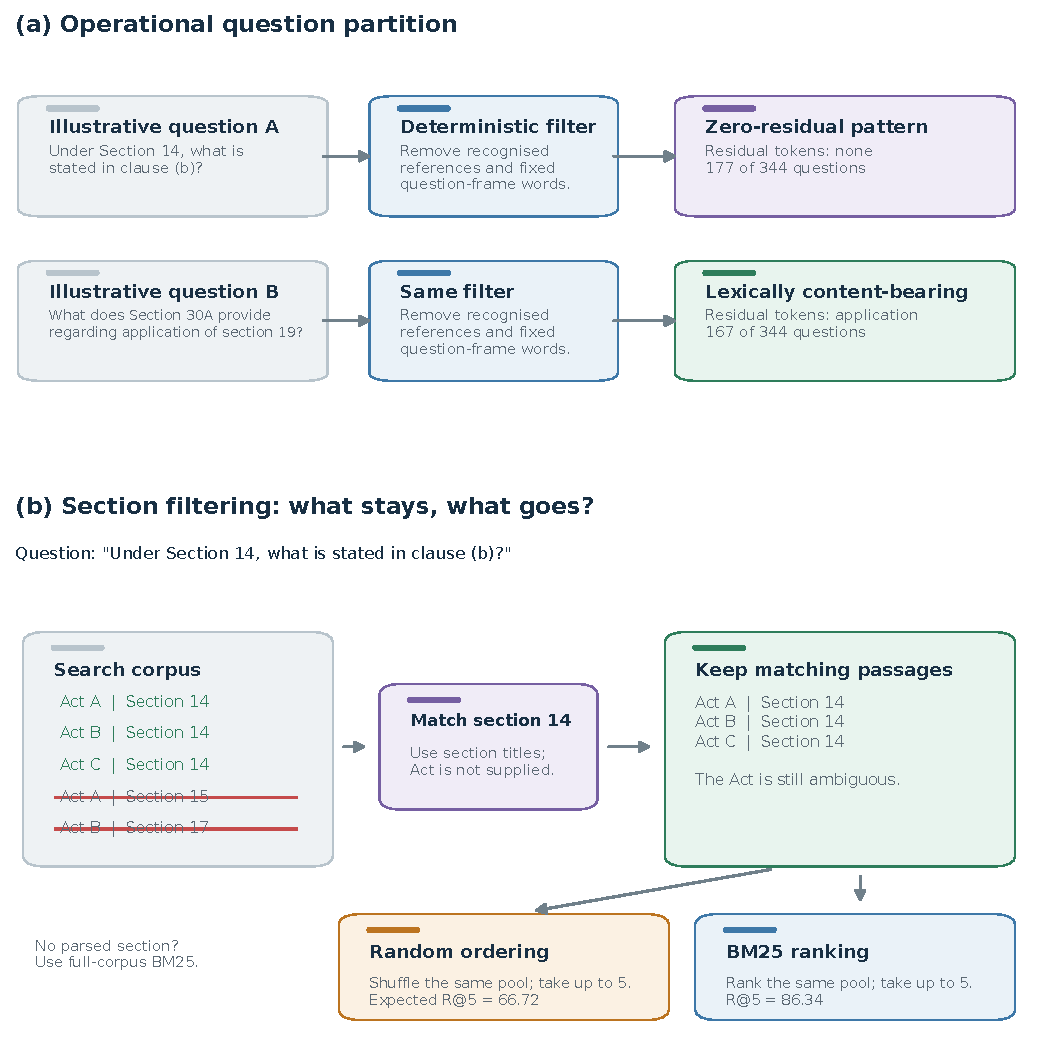
\includegraphics[width=\textwidth]
    {plots/01_retrieval_diagnostic_overview.pdf}
    \caption{Main rules used in the analysis. Panel (a) shows how the text rule
    separates zero-residual reference-pattern questions from lexically
    content-bearing questions. Panel (b) shows how a Section 14 reference keeps
    passages with the same section number from different Acts and removes other
    sections. Random ordering and BM25 ranking use the same matched pool. Both
    methods keep all passages when fewer than five match. The recall@5 values
    summarise all 344 test questions and do not refer only to the example.
    Questions without a parsed section use BM25 as a fallback.}
    \label{fig:study_pipeline_overview}
\end{figure}

\FloatBarrier

\subsection{IndicIPR-QA}
\label{sec:dataset_description}

IndicIPR-QA is an extractive QA benchmark with 4,462 question--answer pairs
from 1,116 statutory paragraphs. It covers seven Acts: the Copyright Act,
1957; Patents Act, 1970; Trade Marks Act, 1999; Designs Act, 2000;
Geographical Indications of Goods (Registration and Protection) Act, 1999;
Semiconductor Integrated Circuits Layout-Design Act, 2000; and Protection of
Plant Varieties and Farmers' Rights Act, 2001
\citep{anonymous2026indiciprqa}.

Each answer is copied from one continuous span in its source paragraph. The
questions were generated by a model and then filtered and curated. The dataset
is split by statute section into 3,710 training, 408 validation, and 344 test
pairs. No supervised context is shared across the three splits.

Dataset validation includes a review of 200 pairs by two annotators. They
assessed question clarity, answer correctness, and answer minimality
\citep{anonymous2026indiciprqa}. Minimality means that the answer contains only
the text needed to answer the question. Dataset construction and validation
are described in a resource paper accepted at IEEE DSAA 2026; its proceedings
entry is forthcoming. This study uses the released splits without changing
them. Access details are provided in the Data and Code Availability statement.

Table~\ref{tab:indicipriqa_stats} reports the main dataset characteristics.

\begin{table}[!htbp]
    \caption{Characteristics of the IndicIPR-QA benchmark used in this study.
    Source: IndicIPR-QA \citep{anonymous2026indiciprqa}.}
    \label{tab:indicipriqa_stats}
    \centering
    \scriptsize
    \begin{tabular}{lr}
        \toprule
        Acts covered                       & 7 \\
        Sections covered                   & 681 \\
        Paragraph-level contexts           & 1,116 \\
        Total QA pairs                     & 4,462 \\
        Train / Validation / Test          & 3,710 / 408 / 344 \\
        Avg.\ context length (words)       & 171.3 \\
        Avg.\ question length (words)      & 11.9 \\
        Avg.\ answer length (words)        & 35.6 \\
        Median answer length (words)       & 28 \\
        Max answer length (words)          & 375 \\
        Answers containing semicolons (\%) & 19.9 \\
        Q--ctx lexical overlap (mean)      & 0.451 \\
        \bottomrule
    \end{tabular}
\end{table}

\FloatBarrier

Two dataset properties are important for this study. First, answers contain
35.6 words on average, so the reader must identify long answer boundaries in
some cases. This fact alone does not show that the task is harder than other
QA tasks. Second, questions identify their target provisions in different
ways. Some describe the content they seek, while others mainly provide a
section or subsection reference. This distinction emerged during the analysis
and was not defined in advance.

\subsection{Gold-Context and Full-Pipeline Evaluation}

In gold-context evaluation, the model receives the annotated paragraph and
only needs to extract an answer. In full-pipeline evaluation, the system first
retrieves candidate paragraphs. The reader then selects one candidate and
extracts an answer from it. Both settings use the same 344 test questions, and
retrieval searches all 1,116 paragraphs in the corpus.

The experiments use the fixed \fixedreader{} reader. It is based on
\texttt{nlpaueb/legal-bert-base-uncased}~\citep{chalkidis2020legalbert}. It was
fine-tuned first on SQuAD~v1 and then on the IndicIPR-QA training split. The
reader reaches 87.37 F1 when it receives the annotated paragraph. Its saved
model and settings remain unchanged across the retrieval experiments. This
allows changes in full-pipeline performance to be examined without changing
the answer reader. The reported source-selection results therefore apply to
this reader and decoder.

The reader was selected from existing configurations after earlier results
were available. It was not selected using a new validation set created for
this study. The study records do not contain a complete list of the alternative
configurations, so their total number is not reported. Keeping the reader fixed
makes the comparisons consistent, but it does not show that the reader is
optimal. The same test questions were used for model selection, error analysis,
and the reference experiments. The results therefore describe a fixed pipeline
on the same questions rather than a new evaluation on unseen data.

The full pipeline has three stages: candidate retrieval, source selection, and
answer extraction. Figure~\ref{fig:qa_pipeline} shows these stages and their
possible failure points.

For each candidate passage, \fixedreader{} predicts one continuous answer span
by scoring possible start and end positions. Long passages are divided into
overlapping windows of 384 tokens with a stride of 128 tokens. Only spans with
a start position that is not after the end position are allowed. The decoder
selects the span with the highest sum of its start and end logits across the
windows.

Logits are the model's scores before they are converted into probabilities.
The main pipeline does not apply a local softmax or calibrate these scores
across passages. The passage with the highest span score is selected as the
source, but this score is not a calibrated estimate of relevance. A passage
divided into more windows also has more opportunities to receive a high score.
The decoder does not correct for this effect. Appendix~\ref{app:review_checks}
reports additional checks of source selection and answer length.

There is no separate limit on answer length, although an answer must fit
within one window. This avoids imposing an arbitrary short-answer limit on a
dataset that contains long annotated answers. However, it does not guarantee
that the predicted boundaries are sensible. The predicted answer is returned
as the corresponding character span from the source paragraph.

Nineteen of the 344 test inputs require more than one window. In 14 of these
cases, the annotated answer is not present in the first window. The same
decoder is used in all main evaluation settings. Two additional controls use
BGE-reranker-v2-m3 to select one passage from either the section-filter
top-five pool or the title-aware neural top-five pool. The fixed reader then
extracts an answer only from that passage. In these controls, raw reader logits
do not select the source.

\begin{landscape}
\begin{figure}[H]
    \centering
    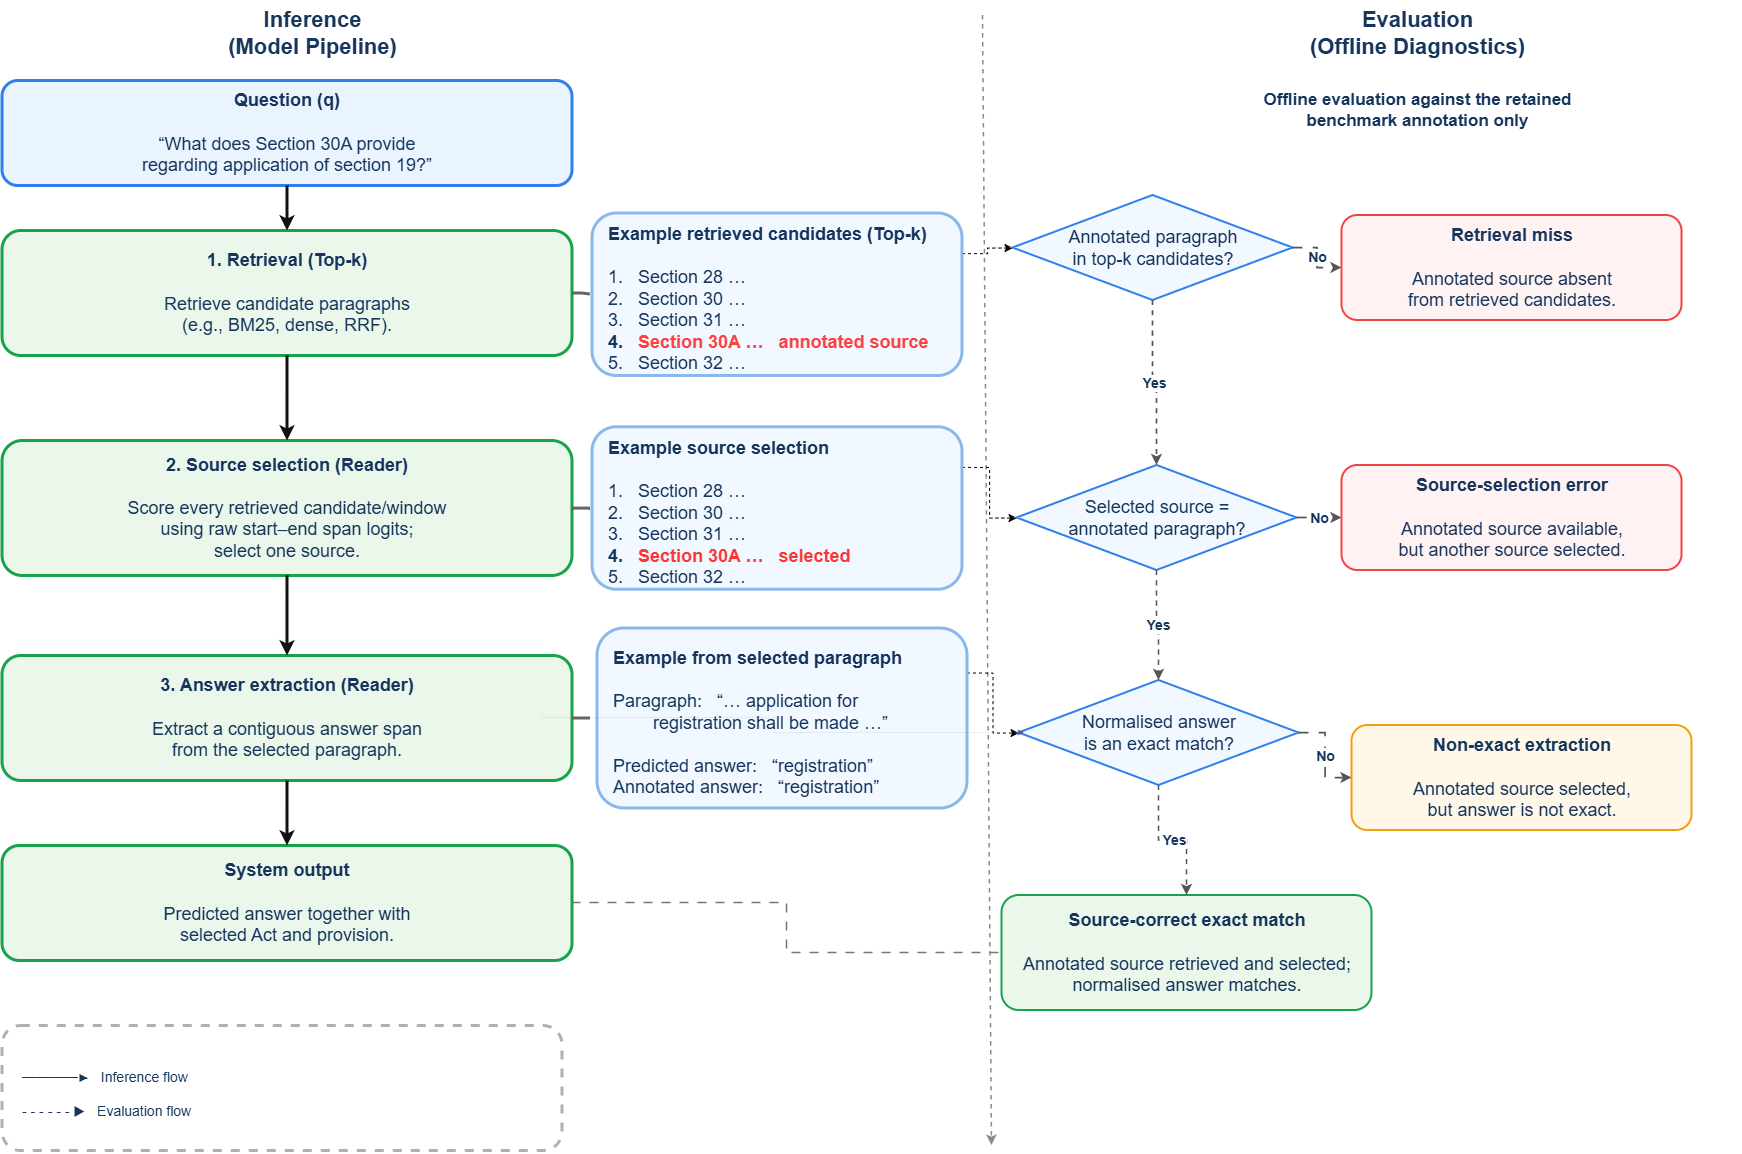
\includegraphics[width=0.82\linewidth]{plots/pipeline1.png}
    \caption{The statutory QA pipeline and its annotation-based diagnostics.
    The left column shows candidate retrieval, reader-based source selection,
    answer extraction, and the final output. The centre column gives an example
    candidate list, selected source, and extracted span. The right column
    compares each stage with the benchmark annotation and assigns one of four
    outcomes: retrieval failure, source-selection failure, non-exact
    extraction, or an exact answer from the annotated source. Solid arrows show
    the inference process, and dashed arrows show offline evaluation. These
    checks do not change inference or establish the legally governing source.}
    \label{fig:qa_pipeline}
\end{figure}
\end{landscape}

Table~\ref{tab:input_specification} shows the information available to each
system. The main BM25, dense, fusion, and cross-encoder experiments use only
paragraph text. The title-aware controls give BM25, BGE-M3, fusion, and BGE
reranking both the section title and paragraph. Section-filtering methods use
titles to create their candidate pools. Annotated Act labels are used only in
oracle controls. These controls either restrict the candidates to the
annotated Act or add the Act name to the query and candidate text.

\begin{table}[!htbp]
    \caption{Input specification for the retrieval and reading systems.
    ``Full question'' means the original benchmark question. Oracle variants
    and fallback rules are described in Table~\ref{tab:metadata_controls}.}
    \label{tab:input_specification}
    \centering
    \scriptsize
    \setlength{\tabcolsep}{3.5pt}
    \begin{tabular}{@{}
        >{\raggedright\arraybackslash}p{2.7cm}
        >{\raggedright\arraybackslash}p{2.5cm}
        >{\raggedright\arraybackslash}p{4.8cm}
        >{\raggedright\arraybackslash}p{2.3cm}@{}}
        \toprule
        Component & Query input & Candidate-side input & Role \\
        \midrule
        BM25 / dense / RRF
        & Full question
        & Paragraph text
        & Content baseline \\

        Cross-encoder
        & Full question
        & Paragraph text for top-50 candidates
        & Reranking \\

        Title+paragraph BM25
        & Full question
        & Section title + paragraph
        & Metadata control \\

        Title-aware BGE / RRF / reranker
        & Full question
        & Section title + paragraph
        & Neural metadata control \\

        Section filter + BM25
        & Parsed section + full question
        & Section titles for matching; paragraph text for ranking
        & Structural diagnostic \\

        Oracle Act restriction
        & Full question
        & Paragraphs from annotated Act
        & Candidate restriction \\

        Oracle Act + section restriction
        & Parsed section + full question
        & Paragraphs from annotated Act and section
        & Candidate restriction \\

        Oracle Act name BM25
        & Full question + annotated Act name
        & Act name + title + paragraph
        & Information-added control \\

        \fixedreader{} reader
        & Full question
        & Paragraph text
        & Answer extraction \\
        \bottomrule
    \end{tabular}
\end{table}

\subsection{Evaluation Metrics}

Normalised Exact Match (EM) and token-level F1 are the main answer-text
metrics. Before scoring, predicted and annotated answers are converted to
lowercase. The ASCII characters in Python's
\texttt{string.punctuation} are removed, and repeated spaces are normalised.
Articles are not removed. This process differs from the official SQuAD
normalisation.

Removing punctuation means that the score may ignore some boundary differences
that are important for legal meaning. However, these differences remain in the
source text and the predicted character span. EM is one when the normalised
prediction exactly matches the normalised reference and zero otherwise:

\begin{equation}
    \mathrm{EM}
    =\mathbf{1}\{\mathrm{norm}(\hat{a})=\mathrm{norm}(a)\},
    \label{eq:em}
\end{equation}

where $a$ is the annotated answer and $\hat{a}$ is the predicted answer.

For token-level F1, let $\mathcal{A}$ and $\mathcal{P}$ be the token
multisets of the annotated and predicted answers. Precision, recall, and F1
are calculated as follows:

\begin{align}
    \mathrm{Precision}
    &= \frac{|\mathcal{A}\cap\mathcal{P}|}{|\mathcal{P}|}, &
    \mathrm{Recall}
    &= \frac{|\mathcal{A}\cap\mathcal{P}|}{|\mathcal{A}|}, \\
    \mathrm{F1}
    &= \frac{2\,\mathrm{Precision}\,\mathrm{Recall}}
    {\mathrm{Precision}+\mathrm{Recall}}.
    \label{eq:f1}
\end{align}

If either token multiset is empty, the implementation assigns an F1 score of
zero. EM requires a complete match after normalisation, while F1 gives partial
credit for shared tokens.

Neither EM nor F1 shows whether the answer came from the annotated paragraph.
The evaluation therefore also reports how often the annotated source is
selected. This is reported both for all questions and for questions where the
source is available in the top five. We also report annotation-grounded EM and
F1. These scores are set to zero when the system selects another paragraph.
Grounded EM is the number of exact answers extracted from the annotated source
in Table~\ref{tab:stage_decomposition}, divided by 344.

These grounded measures use benchmark annotations. They are not expert
judgements that the annotated paragraph is the only legally correct source.
Character-frequency overlap is not used because it ignores character order and
can give high scores to legally different answers. Appendix~\ref{app:secondary}
describes the older artifact field that stores this unused measure.

\subsection{Human Evaluation Protocol}
\label{sec:human_protocol}

The human audit examines the section-filter top-five pipeline with the original
raw-logit decoder. Using random seed 42, we sampled 20 questions without
replacement from each of four pipeline outcomes:

\begin{enumerate}[label=(\roman*)]
    \item the annotated source was absent;
    \item the annotated source was available but another source was selected;
    \item the annotated source was selected but the answer was not an exact
    match; and
    \item the annotated source was selected and the answer was an exact match.
\end{enumerate}

These four groups contain 47, 122, 44, and 131 questions in the full test set.
The audit therefore covers 80 of the 344 test questions. Each group contributes
20 cases even though the groups have different sizes in the full test set.
Results are reported separately for each group. Combining the 80 cases without
weights would not estimate the frequency of legal errors in the full test set.

Two law graduate students, identified only by anonymised codes in this paper,
assessed the cases separately and then discussed them to reach agreed labels.
The task was limited to comparing the supplied questions, statutory passages,
and answer spans. It did not ask the reviewers to provide legal advice,
determine the current governing law, or represent practitioner consensus. Both
reviewers knew that their assessments would be used in this research and agreed
to that use.

No AI-generated draft assessments were shown to the reviewers during
annotation or consensus. This restriction concerned annotation suggestions,
not the system predictions that they assessed. Each form showed the question,
two statutory passages with their Act names and titles, and the related
answers. The labels A and B hid which passage and answer came from the
benchmark and which came from the system. These labels were not reviewer
identifiers.

The forms did not collect a separate judgement based only on the question.
When reviewers assessed whether a question identified a unique source, they
could see both candidate passages. They did not freely search the complete
statutory corpus.

The reviewers assessed source identifiability, legal relevance, legal
equivalence between the sources, answer correctness, error materiality, and
text quality. Error materiality describes how strongly an error changes the
legal meaning of an answer. The assessment was limited to the archived
passages shown in the forms and did not verify the current law.

The same two reviewers recorded the final labels, reasons, discussion notes,
and confirmations. There was no third adjudicator. The original separate
ratings are retained for agreement analysis and are kept separate from later
revisions and consensus labels.

Raw agreement, Cohen's nominal $\kappa$ \citep{cohen1960agreement}, Gwet's
AC1~\citep{gwet2008agreement}, and quadratic weighted materiality
$\kappa$~\citep{cohen1968weighted} are reported as descriptive measures of
reviewer consistency. They are not tests of legal validity.
Appendix~\ref{app:human_agreement} describes the categories, denominators, and
excluded cases.


\FloatBarrier


%% ============================================================
\section{Establishing the Retrieval--Reading Gap}
\label{sec:results}

Following the evaluation protocol in Section~\ref{sec:experimental_setup},
BM25 searches the 1,116 statutory paragraphs and returns the top-$k$
candidates. The fixed reader, \fixedreader{}, extracts an answer span from
each candidate. The system then selects the paragraph containing the answer
span with the highest raw reader span score:
\begin{align}
    \hat{c}
    &= \argmax_{c\in \mathrm{Top}_k(q)} S_{\theta}(q,c), \\
    \hat{a}
    &= a_{\theta}(q,\hat{c}).
    \label{eq:retrieve_read}
\end{align}
Here, $\mathrm{Top}_k(q)$ is the set of top-$k$ paragraphs returned by BM25.
For each paragraph $c$, $S_{\theta}(q,c)$ is the maximum summed raw
start--end logit score across all valid answer spans and input windows. The
function $a_{\theta}(q,\hat{c})$ returns the answer span corresponding to this
score. Further details about BM25 are provided in
Appendix~\ref{app:secondary}.

\begin{table}[!ht]
    \caption{Annotated-source recall and extractive QA performance using
    \fixedreader{} on IndicIPR-QA.}
    \label{tab:end_to_end_retrieval_qa}
    \centering
    \small
    \setlength{\tabcolsep}{4pt}
    \begin{tabular}{lccc}
        \toprule
        Setting & \shortstack{Annotated-source\\recall (\%)} &
        EM (\%) & F1 (\%) \\
        \midrule
        Annotated paragraph + \fixedreader{} & 100.00 & 66.86 & 87.37 \\
        BM25 top-1 + \fixedreader{}           & 13.08  & 10.76 & 29.47 \\
        BM25 top-3 + \fixedreader{}           & 20.06  & 11.34 & 31.04 \\
        BM25 top-5 + \fixedreader{}           & 22.67  & 10.47 & 31.95 \\
        \bottomrule
    \end{tabular}
\end{table}

Table~\ref{tab:end_to_end_retrieval_qa} shows the retrieval-reading gap.
F1 falls from 87.37 when the annotated paragraph is given to the reader to
31.95 when the reader uses the top five paragraphs returned by BM25.
BM25 retrieves the annotated paragraph in its top five results for only
22.67\% of the questions. Increasing the candidate pool from one paragraph
to five improves F1 by only 2.48 points. These results show why candidate
retrieval, source selection, and answer extraction should be examined
separately.

The annotated paragraph is missing from BM25's top five results for 266
questions. In 188 of these cases, BM25's top-ranked paragraph comes from a
different Act. In the other 78 cases, it comes from the annotated Act but is
not the annotated paragraph. These counts describe whether BM25's top-ranked
source matches the Act of the benchmark annotation. They do not show whether
another paragraph is legally relevant or how serious the difference may be.
The reader has no option to return ``no answer.'' It therefore extracts an
answer from one of the retrieved paragraphs even when the annotated paragraph
is missing (Sections~\ref{sec:qualitative} and~\ref{sec:limitations}).

\section{Content-Based Retrieval and Reranking}
\label{sec:content_retrieval}

\subsection{Sparse, Dense, and Hybrid Initial Retrieval}
\label{sec:dense_retrieval}

The BM25 results raise the question of whether other content-based retrievers
can recover annotated paragraphs missed by BM25. This experiment compares four
zero-shot dense retrievers and sparse--dense fusion using the same 1,116
passages and 344 test questions. The dense models independently encode each
question and passage and rank passages by cosine similarity. Reciprocal rank
fusion (RRF, $k{=}60$)~\citep{cormack2009rrf} combines the BM25 and E5
rankings. E5 has the highest recall@5 among the four dense models.

All content-based systems use paragraph text only. They do not receive section
titles, section fields, or Act labels. Dense embeddings are L2-normalised. The
models use their standard query and passage prefixes where required, a batch
size of 32, and default truncation. The RRF results in
Table~\ref{tab:dense_retrieval} use depth-10 rankings from BM25 and E5. The
depth-50 fusion used for cross-encoder reranking is reported separately.

\begin{table}[!htbp]
    \caption{Annotated-source retrieval on 1,116 statutory passages and 344
    test questions. All scores are on the 0--100 scale.}
    \label{tab:dense_retrieval}
    \centering
    \scriptsize
    \setlength{\tabcolsep}{3pt}
    \begin{tabular}{@{}lrrrrr@{}}
        \toprule
        Retriever & R@1 & R@3 & R@5 & R@10 & MRR@10 \\
        \midrule
        BM25 (sparse)                & 13.08 & 20.06 & 22.67 & 27.03 & 17.34 \\
        \midrule
        all-MiniLM-L6-v2             & 10.17 & 16.28 & 20.93 & 28.20 & 14.70 \\
        multi-qa-MiniLM-L6-cos-v1    &  8.43 & 16.28 & 17.73 & 24.13 & 12.66 \\
        bge-small-en-v1.5            & 10.17 & 18.31 & 22.38 & 30.23 & 15.80 \\
        e5-small-v2                  &  9.88 & 18.31 & 23.26 & 29.94 & 15.60 \\
        \midrule
        Hybrid RRF (BM25 + E5)       & 11.92 & 19.77 & 26.16 & 31.40 & 17.47 \\
        \bottomrule
    \end{tabular}
    \begin{flushleft}
        {\scriptsize All rows use the same retrieval-only pipeline. The
        canonical BM25 ordering sorts passages by descending score and then
        by ascending index in the released paragraph corpus. BM25 uses
        $k_1{=}1.5$ and $b{=}0.75$. A legacy script used a different corpus
        order. The identity-matched comparison is reported in
        Appendix~\ref{app:review_checks}.}
    \end{flushleft}
\end{table}

No dense model outperforms BM25 on every reported metric in
Table~\ref{tab:dense_retrieval}. E5 gives the highest recall@5 among the four
dense models, while BM25--E5 fusion gives the highest overall recall@5 in this
initial comparison, at 26.16. These zero-shot results do not show how a legally
supervised retriever would perform. A separate extension using larger modern
models is presented after the reranking baseline.

\FloatBarrier

\subsection{Does Cross-Encoder Reranking Help?}
\label{sec:reranking}

Initial retrieval may fail in two ways. First, the annotated paragraph may be
missing from the candidate pool. Second, it may be present but ranked too low.
This experiment examines the second case. BM25 and the hybrid retriever each
provide 50 candidates to the Sentence Transformers checkpoint
\texttt{ms-marco-MiniLM-L6-v2}.\footnote{Model card:
\url{https://huggingface.co/cross-encoder/ms-marco-MiniLM-L6-v2}.
The archived experiment code uses the older \texttt{L-6} identifier.}
The cross-encoder scores each question and passage together. Its maximum input
length is 512 tokens, and its batch size is 64. The corpus, test questions,
and annotated-source matching remain unchanged. Recall@50 is the highest
recall that the reranker can achieve because it cannot recover an annotated
paragraph that is absent from the initial candidate pool.

\enlargethispage{27pt}% Accommodate the checkpoint footnote without a vertical overflow.

\begin{table}[!htbp]
    \caption{Cross-encoder reranking of the top 50 initial candidates.
    Recall@50 is the maximum recall available to the reranker.
    All scores are on the 0--100 scale.}
    \label{tab:rerank}
    \centering
    \scriptsize
    \setlength{\tabcolsep}{3pt}
    \begin{tabular}{@{}lrrrrrr@{}}
        \toprule
        System & R@1 & R@3 & R@5 & R@10 & R@50 & MRR@10 \\
        \midrule
        BM25                   & 13.08 & 20.06 & 22.67 & 27.03 & 41.86 & 17.34 \\
        \quad + cross-encoder  & 17.44 & 26.45 & 29.94 & 34.59 & 41.86 & 22.56 \\
        Hybrid RRF             & 11.92 & 22.09 & 26.74 & 33.72 & 40.41 & 18.12 \\
        \quad + cross-encoder  & 17.15 & 24.71 & 30.23 & 35.17 & 40.41 & 22.30 \\
        \bottomrule
    \end{tabular}
    \begin{flushleft}
        {\scriptsize The hybrid rows differ slightly from
        Table~\ref{tab:dense_retrieval} because fusion is computed over
        depth-50 rather than depth-10 rankings. All other settings remain
        unchanged.}
    \end{flushleft}
\end{table}

Cross-encoder reranking raises BM25 recall@5 from 22.67 to 29.94
(Table~\ref{tab:rerank}). The hybrid pipeline reaches 30.23 recall@5.
However, the initial recall@50 values are only 41.86 for BM25 and 40.41 for
the hybrid retriever. Therefore, most annotated paragraphs remain outside
the candidate pools and cannot be recovered through reranking.

To test whether these findings are limited to the smaller checkpoints, a
separate modern-model extension evaluates dense BGE-M3
\citep{chenM3Embedding2024} and BGE-reranker-v2-m3.\footnote{Model card:
\url{https://huggingface.co/BAAI/bge-reranker-v2-m3}.}
Both checkpoints are used without legal-domain fine-tuning. The first
comparison uses paragraph text alone. A matched comparison then adds the
section title before each paragraph and repeats BM25, BGE-M3, fusion, and
reranking. The maximum sequence length is 512 tokens. BGE-M3 embeddings are
L2-normalised. RRF combines depth-50 BM25 and BGE-M3 rankings using $k=60$.
The BGE reranker reorders the first 50 candidates provided by BM25 or RRF.
The archived manifest records the exact checkpoint revisions and runtime
settings.

\begin{table}[!htbp]
    \caption{Modern-model retrieval extension on IndicIPR-QA. The lower panel
    repeats the comparison with section titles prepended to the candidate
    paragraphs. Reranking preserves the recall@50 ceiling of the initial
    candidate pool. All scores are on the 0--100 scale.}
    \label{tab:modern_bge_indic}
    \centering
    \scriptsize
    \renewcommand{\arraystretch}{0.93}
    \setlength{\tabcolsep}{1.3pt}
    \begin{tabular}{@{}lrrrrrrr@{}}
        \toprule
        System & R@1 & R@3 & R@5 & R@10 & R@50 & MRR@10 & nDCG@10 \\
        \midrule
        BM25 & 13.08 & 20.06 & 22.67 & 27.03 & 41.86 & 17.34 & 19.66 \\
        BGE-M3 & 14.24 & 20.93 & 29.94 & 33.72 & 46.22 & 19.51 & 22.87 \\
        BM25 + BGE-M3 RRF & 14.24 & 24.71 & 30.81 & 36.05 & 45.06 & 20.72 & 24.39 \\
        BM25 + BGE reranker & 18.02 & 25.58 & 29.07 & 33.72 & 41.86 & 22.69 & 25.33 \\
        BGE RRF + BGE reranker & 17.73 & 25.58 & 29.36 & 34.01 & 45.06 & 22.76 & 25.46 \\
        \midrule
        Title+paragraph BM25 & 34.88 & 47.97 & 56.98 & 69.77 & 94.77 & 44.56 & 50.48 \\
        Title+paragraph BGE-M3 & 34.01 & 46.22 & 52.03 & 60.76 & 81.40 & 42.17 & 46.59 \\
        Title+paragraph RRF & 45.35 & 61.05 & 70.64 & 77.91 & 94.48 & 55.21 & 60.66 \\
        Title+paragraph RRF + BGE reranker & 51.74 & 75.29 & 83.72 & 91.28 & 94.48 & 65.46 & 71.72 \\
        \bottomrule
    \end{tabular}
\end{table}

Table~\ref{tab:modern_bge_indic} compares both the retrieval models and the
information provided to them. With paragraph text alone, BGE-M3 raises
recall@5 from 22.67 for BM25 to 29.94. BM25--BGE-M3 fusion reaches 30.81
recall@5. Its recall@50 ceiling is 45.06, so the annotated paragraph remains
outside the top five for 69.19\% of the questions.

Adding section titles produces much higher retrieval scores. Title-plus-
paragraph fusion reaches 70.64 recall@5, and BGE reranking raises it to
83.72. The reranker works within the fused candidate pool, which has a
recall@50 ceiling of 94.48. This controlled comparison shows that passage
representation is a major factor in the retrieval results. The tested neural
models can use section-title information when it is provided.

The strongest title-aware neural configuration and the title-plus-paragraph
BM25 control are also evaluated with the fixed answer reader in
Section~\ref{sec:section_end_to_end}. The title-aware BGE-M3 and unre-ranked
RRF configurations are retrieval-only comparisons.

Results by Act provide further motivation for the question analysis in the
next section. Plant Varieties reaches 72.50 recall@5 with the depth-50 hybrid
pipeline followed by cross-encoder reranking. Designs remains at 0.00
recall@5 because its annotated paragraphs are absent from the initial
candidate pool (Table~\ref{tab:retrieval_per_act}). Because the hybrid
pipeline changes both initial retrieval and reranking, this comparison does
not isolate the effect of reranking. Together with the contrast between
paragraph-only and title-aware retrieval, these Act-level results motivate
the structural diagnosis in the next section.


\section{Diagnosing Zero-Residual Reference Patterns}
\label{sec:structural_diagnosis}

This section examines whether retrieval difficulty is associated with question wording. It first compares reading and retrieval performance across Acts. It then uses an operational text rule to divide the questions into zero-residual and lexically content-bearing groups and compares their performance. The analysis is exploratory, and the groups are defined by a text rule rather than expert semantic judgements.

\subsection{Act-Level Differences in Reading and Retrieval}
\label{sec:per_act_clue}

Results for individual Acts show a contrast between reading and retrieval
performance (Table~\ref{tab:retrieval_per_act}). For Designs, F1 reaches
98.97 when the annotated paragraph is provided, while recall@5 remains 0.00
for all three retrieval pipelines. In contrast, Plant Varieties has the
highest recall@5 in all three retrieval columns but the lowest
annotated-paragraph F1, at 72.26.

\begin{table}[!htbp]
    \caption{Recall@5, question--context lexical overlap, and
    annotated-paragraph F1 by Act. Reading and retrieval show contrasting
    patterns. The final retrieval column uses the hybrid pipeline with
    cross-encoder reranking described in Section~\ref{sec:reranking}.
    Recall and F1 are on the 0--100 scale; lexical overlap is on the
    0--1 scale.}
    \label{tab:retrieval_per_act}
    \centering
    \scriptsize
    \setlength{\tabcolsep}{3pt}
    \begin{tabular}{@{}lrrrrr@{}}
        \toprule
        Act & Q--Ctx overlap & BM25 R@5 & Hybrid R@5 &
        Hybrid+CE R@5 & Reader F1 \\
        \midrule
        Plant Varieties & 0.636 & 45.00 & 50.00 & 72.50 & 72.26 \\
        Copyright       & 0.447 & 32.00 & 36.00 & 36.00 & 74.57 \\
        GI              & 0.458 & 25.49 & 31.37 & 35.29 & 83.62 \\
        Patents         & 0.429 & 24.64 & 23.19 & 26.09 & 96.34 \\
        Trade Marks     & 0.416 & 17.05 & 22.73 & 21.59 & 86.32 \\
        Semiconductor   & 0.418 & 14.89 & 19.15 & 23.40 & 94.00 \\
        Designs         & 0.320 &  0.00 &  0.00 &  0.00 & 98.97 \\
        \bottomrule
    \end{tabular}
    \begin{flushleft}
        {\scriptsize The Hybrid column combines depth-10 BM25 and
        \texttt{e5-small-v2} rankings using RRF ($k=60$). Hybrid+CE combines
        depth-50 BM25 and E5 rankings, retains the 50-candidate pool, and
        reranks it with \texttt{ms-marco-MiniLM-L-6-v2}. Both pipelines use
        paragraph text only and search the same 1,116-passage corpus.}
    \end{flushleft}
\end{table}

These results show that questions that are difficult for retrieval are not
necessarily difficult for the reader when the annotated paragraph is
provided. Many Designs questions mainly contain statutory locators, such as
``Under Section 7'', and provide few distinctive terms for retrieval from
paragraph text alone. The within-Act comparisons below examine whether the
difference between question groups also appears within individual Acts.

\subsection{Question Groups Defined by a Text Rule}
\label{sec:citation_specified}

The Act-level results motivate a closer examination of question wording.
This analysis is exploratory because the question groups were developed after
examining the test material. They were not defined before evaluation.

A fixed text rule removes recognised section, subsection, clause, item, and
paragraph references, together with a fixed list of question-frame words.
Questions with no remaining tokens are classified as a
\emph{zero-residual reference pattern} ($n=177$). The tables use
\emph{zero-residual} as a shorter name for the same group. Questions with one
or more remaining tokens are classified as \emph{lexically content-bearing}
($n=167$). These labels describe the result of the text rule. They are not
expert judgements about the meaning of a question, and a zero-residual
question may still have legal meaning. Appendix~\ref{sec:classifier_robustness}
provides the full rule, the word list, and checks using different token
thresholds.

\begin{table}[!htbp]
    \caption{Answer scores for the two test-question groups defined by the
    text rule. The same fixed reader is used in both settings.}
    \label{tab:citation_specified}
    \centering
    \small
    \setlength{\tabcolsep}{4pt}
    \begin{tabular}{@{}lrcccc@{}}
        \toprule
        & & \multicolumn{2}{c}{Annotated paragraph} &
        \multicolumn{2}{c}{BM25 top-5 + reader} \\
        \cmidrule(lr){3-4}\cmidrule(lr){5-6}
        Question type & $n$ & EM (\%) & F1 (\%) & EM (\%) & F1 (\%) \\
        \midrule
        Zero-residual pattern     & 177 & 74.01 & 91.55 &  0.00 & 17.59 \\
        Lexically content-bearing & 167 & 59.28 & 82.94 & 21.56 & 47.17 \\
        \midrule
        All                       & 344 & 66.86 & 87.37 & 10.47 & 31.95 \\
        \bottomrule
    \end{tabular}
    \begin{flushleft}
        {\scriptsize The primary rule classifies a question as zero-residual
        when no tokens remain after removing recognised statutory references
        and fixed question-frame words. The labels are operational, not human
        semantic annotations.}
    \end{flushleft}
\end{table}

For the zero-residual group, F1 falls from 91.55 with the annotated paragraph
to 17.59 when BM25 top-five retrieval is followed by the fixed reader. This
group has no exact matches in the full pipeline. In comparison, the
lexically content-bearing group reaches 47.17 F1 in the same full-pipeline
setting (Table~\ref{tab:citation_specified}).

The two groups are not defined only by whether a citation is present. Among
the 167 lexically content-bearing questions, 148 contain both a parsable
statutory citation and residual lexical tokens. The other 19 have no parsable
citation. The distribution across Acts and the possible effects of question
generation are discussed in Appendix~\ref{app:secondary}.

Differences in the numbers of questions from each Act do not fully explain
the overall result. Five Acts have at least nine questions in each group.
Within all five Acts, BM25 recall@5 is 0.00 for the zero-residual group. For
the lexically content-bearing group, it ranges from 30.43 to 88.89
(Table~\ref{tab:within_act_question_groups}). However, these comparisons do
not rule out effects of question generation or question difficulty.

The results therefore show an association between the zero-residual reference
pattern and difficulty in recovering the annotated source on this benchmark.
They do not establish that statutory references alone cause annotated-source
retrieval failures.

\FloatBarrier



%% ============================================================
\section{Candidate Filtering Using Section References}
\label{sec:citation_rq}

Following the question-wording analysis in RQ2, this section addresses RQ3
by examining how statutory references affect retrieval of the annotated
source. It also examines how changes in the candidate pool affect source
selection and answer extraction.

\subsection{Section Matching Rule and Metadata Controls}
\label{sec:citation_aware}

This experiment evaluates section matching. Separate controls examine the
contributions of passage titles, candidate-pool size, and ranking within the
candidate pool.

Each passage title begins ``Section~$n$: \ldots''. A regular expression
extracts the first section identifier from the question and from each passage
title. The rule does not use relevance labels, passage identities, or the
annotated Act. No question names its target Act, and section numbers recur
across Acts. The rule extracts a section identifier for 94.48\% of the test
questions. This percentage is not a human-validated estimate of parser
accuracy. Here, \emph{citation} means an internal statutory locator.

The exact case-insensitive pattern is
\begin{quote}\small
\verb|\bsections?\s*[.\-]?\s*(\d+[A-Za-z]{0,2})\b|
\end{quote}
The system converts the first match to uppercase and compares it with the
first section identifier in each title. The rule accepts letter suffixes.
It does not use subsection or clause locators to distinguish passages that
share a section number, expand ranges or lists, or determine which of several
references is legally controlling. Examples and item-level disagreements are
reported in Appendix~\ref{app:review_checks}.

Of the 325 parsed first references, 321 agree with the section of the
annotated source. The four disagreements and 19 unparsed cases are left
unchanged; source labels are not used to correct them
(Appendix~\ref{app:review_checks}). This agreement does not establish parser
accuracy, identify the intended source, or show that the source is unique.

The filter is query-driven rather than an annotation oracle. It uses the
locator written in the question without access to the annotated Act or
paragraph identity. However, it is a structurally privileged setting because
it relies on an explicit, parsable section locator when one is available.
Section filtering is therefore evaluated as a diagnostic intervention,
together with title, random-pool, wrong-locator, predicted-Act, and oracle-Act
controls. It is not presented as a general replacement for content retrieval.

Two structural methods are evaluated. The \emph{boost} adds 1,000 BM25-score
units to passages from the parsed section and then ranks the full corpus.
The \emph{filter} uses BM25 on paragraph text to rank only passages from the
parsed section. It returns all matching passages when fewer than five are
available. If no matching passage is found, including when no section is
parsed, the system falls back to unrestricted BM25. Both methods rank by
descending score and use ascending corpus index to break ties.

Boosting and filtering achieve the same recall@1, recall@3, and recall@5:
50.29, 73.26, and 86.34, respectively. However, their top-five candidate
sets differ for 73 questions because boosting fills pools with fewer than
five section matches using passages from the full corpus. The reader selects
different passages for 20 questions. For this subgroup, filtering increases
reader F1 by 13.06 points. The increase is 2.77 points across all 344
questions. At rank 10, recall is 95.64 for boosting and 95.35 for filtering.
The filter uses unrestricted BM25 as a fallback for the 19 unparsed
questions.

Table~\ref{tab:citation_aware} compares the aggregate retrieval performance
of section boosting with the content-based retrieval baselines.

\begin{table}[!htbp]
    \caption{Section-reference retrieval and content-based retrieval on the
    same 1,116 passages and 344 test questions. Section boosting is
    deterministic. All scores are on the 0--100 scale.}
    \label{tab:citation_aware}
    \centering
    \scriptsize
    \setlength{\tabcolsep}{4pt}
    \begin{tabular}{@{}lrrrrr@{}}
        \toprule
        System & R@1 & R@3 & R@5 & R@10 & MRR@10 \\
        \midrule
        BM25                           & 13.08 & 20.06 & 22.67 & 27.03 & 17.34 \\
        BM25 + BGE-M3 RRF              & 14.24 & 24.71 & 30.81 & 36.05 & 20.72 \\
        BGE RRF + BGE reranker         & 17.73 & 25.58 & 29.36 & 34.01 & 22.76 \\
        \midrule
        Section boost + paragraph BM25 & 50.29 & 73.26 & 86.34 & 95.64 & 64.84 \\
        \bottomrule
    \end{tabular}
    \begin{flushleft}
        {\scriptsize The BGE rows reproduce the depth-50 modern-model
        extension in Table~\ref{tab:modern_bge_indic}. The BGE reranker
        cannot change the 45.06 recall@50 ceiling of its RRF candidate pool.}
    \end{flushleft}
\end{table}

\begin{table}[!htbp]
    \caption{Metadata and candidate-pool controls on the 344 test questions.
    The random-order values separate candidate-pool reduction from ranking.
    The section-pool value is the expected recall@5; the value in parentheses
    is the mean $\pm$ standard deviation from a simulation of 10,000 random
    orders. Oracle rows use the annotated Act. They are diagnostic controls,
    not deployable baselines.}
    \label{tab:metadata_controls}
    \centering
    \scriptsize
    \setlength{\tabcolsep}{5pt}
    \begin{tabular}{@{}lr@{}}
        \toprule
        Control & R@5 (\%) \\
        \midrule
        Paragraph BM25 & 22.67 \\
        Title+paragraph BM25 & 56.98 \\
        Same-size corpus pool, random order & 3.86 \\
        Section pool, random order & 66.72 (66.72 $\pm$ 2.07) \\
        Section filter, paragraph ranker & 86.34 \\
        Section filter, title+paragraph ranker & 87.50 \\
        Predicted Act+section, hard filter & 75.00 \\
        Predicted Act+section, empty-pool fallback & 77.91 \\
        Oracle Act restriction, paragraph ranker & 35.17 \\
        Oracle Act name query, title+paragraph ranker & 79.07 \\
        Oracle Act+section restriction, paragraph ranker & 96.80 \\
        Oracle Act+section, title ranker with Act name fallback & 97.09 \\
        \bottomrule
    \end{tabular}
    \begin{flushleft}
        {\scriptsize Title+paragraph controls add passage titles to BM25.
        In full-pipeline evaluations, the reader still receives paragraph
        text only. The same-size corpus control samples as many passages as
        the matching section pool but does not use the section identifier.
        \emph{Restriction} leaves the question unchanged and limits candidates
        using the annotated Act. \emph{Act name query} adds the Act name to
        both the query and candidate representations. The final row ranks
        titles and paragraphs within the annotated Act and parsed section.
        When no section is parsed, it uses the full-corpus Act-name query
        control rather than Act restriction. Predicted Act+section uses a
        question-only Act classifier trained on the training split and does
        not use the annotated Act at retrieval time.}
    \end{flushleft}
\end{table}

Adding section titles raises BM25 recall@5 from 22.67 to 56.98, while section
filtering reaches 86.34. Adding titles to the ranking within the section pool
raises recall@5 by only 1.16 points, from 86.34 to 87.50
(Table~\ref{tab:metadata_controls}). Title information therefore explains
part of the gap between paragraph-only BM25 and section filtering.

The stronger representation-matched comparison in
Table~\ref{tab:modern_bge_indic} reduces the remaining difference.
Title-plus-paragraph fusion with BGE reranking reaches 83.72 recall@5, which
is 2.62 points below section filtering. Section matching remains a useful
diagnostic signal, but the large paragraph-only gap does not show that strong
retrievers cannot use title metadata. Only 19 questions have no parsable
section reference. These results therefore do not establish that section
filtering is broadly effective for questions without statutory locators.
They measure the value of locators available in this question set and the
candidate pools produced from them.

For a parsed query with a nonempty section pool \(C_i\), expected top-five
annotated-source recovery under random ordering is
\[
p_i=\mathbf{1}\{g_i\in C_i\}\min(1,5/|C_i|),
\qquad
\mathbb{E}[\mathrm{R@5}]
=\frac{100}{344}\sum_{i=1}^{344}p_i.
\]
Here, \(g_i\) is the annotated paragraph. For a query that uses fallback,
\(p_i\) is the fixed unrestricted-BM25 top-five hit indicator. The 19
unparsed questions therefore do not receive random full-corpus rankings.

The section-matched pool contains 7.89 passages on average, with a median of
8 and a range of 1--15. Among the 325 parsed queries, 82 have at most five
matches and 243 have more than five. Random ordering of these pools gives
an expected recall@5 of 66.72. A simulation of 10,000 random orders also
gives 66.72, with an SD of 2.07 and a 95\% simulation range of
$[62.79,70.93]$.

BM25 ranking within the same pools reaches 86.34 recall@5. This is 19.62
points higher than expected random ordering, with a paired source-cluster
95\% interval of $[13.73,25.46]$. A separate size-only control samples
random pools of the same size from the full corpus and reaches only 3.86
recall@5. Candidate-pool size alone therefore does not explain the
section-filter result. Section matching increases access to the annotated
paragraph, while BM25 helps rank that paragraph within the matched pool.
This does not establish section filtering as a general retrieval method
because it uses section identifiers already present in these questions.

Figure~\ref{fig:retrieval_progression} summarises the retrieval progression
and the differences between the two operational question groups.

Oracle Act restriction raises BM25 recall@5 to 35.17, while oracle Act and
section restriction reaches 96.80. The Act-name query control reaches 79.07
by also changing the query and candidate text. These comparisons are
diagnostic controls, not deployable baselines.

A further test examines whether predicting the Act improves section filtering
without using annotated Act labels at retrieval time. A TF--IDF
logistic-regression classifier was trained using question text and Act labels
from 3,691 training pairs. Before training, 19 pairs whose question text
exactly matched a validation or test question were removed. The classifier
was not tuned or refitted on validation or test data. It achieves 81.37\%
Act accuracy on validation and 78.20\% on test.

Restricting the parsed section pool to the predicted Act lowers test
recall@5 from 86.34 to 75.00. Allowing an empty intersection to fall back to
the section pool gives 77.91 recall@5. This loss is consistent with incorrect
Act predictions removing the annotated paragraph from the candidate pool.
The results do not support adding this simple Act classifier to the section
filter.

A locator-sensitivity check replaces each parsed section number with a
different valid number chosen without using the annotated Act or source.
None of the 325 parsed questions retains the annotated paragraph in the
resulting top five. Overall recall@5 is 3.49 because the 19 unparsed questions
retain the usual BM25 fallback, which provides all 12 hits. This result is
expected for a hard section filter. It shows that retrieval is sensitive to
the locator; it does not show that the system has learned legal reasoning.

For the zero-residual reference-pattern group, oracle Act restriction raises
BM25 recall@5 from 0.00 to 5.65 and section-filter recall@5 from 83.62 to
100.00. For the lexically content-bearing group, it raises BM25 recall@5
from 46.71 to 66.47 and section-filter recall@5 from 89.22 to 93.41.
For section filtering, oracle Act restriction closes a larger gap for the
zero-residual group, at 16.38 points, than for the lexically content-bearing
group, at 4.19 points. This pattern is consistent with greater cross-Act
ambiguity when descriptive wording is absent.

\begin{figure}[!htbp]
    \centering
    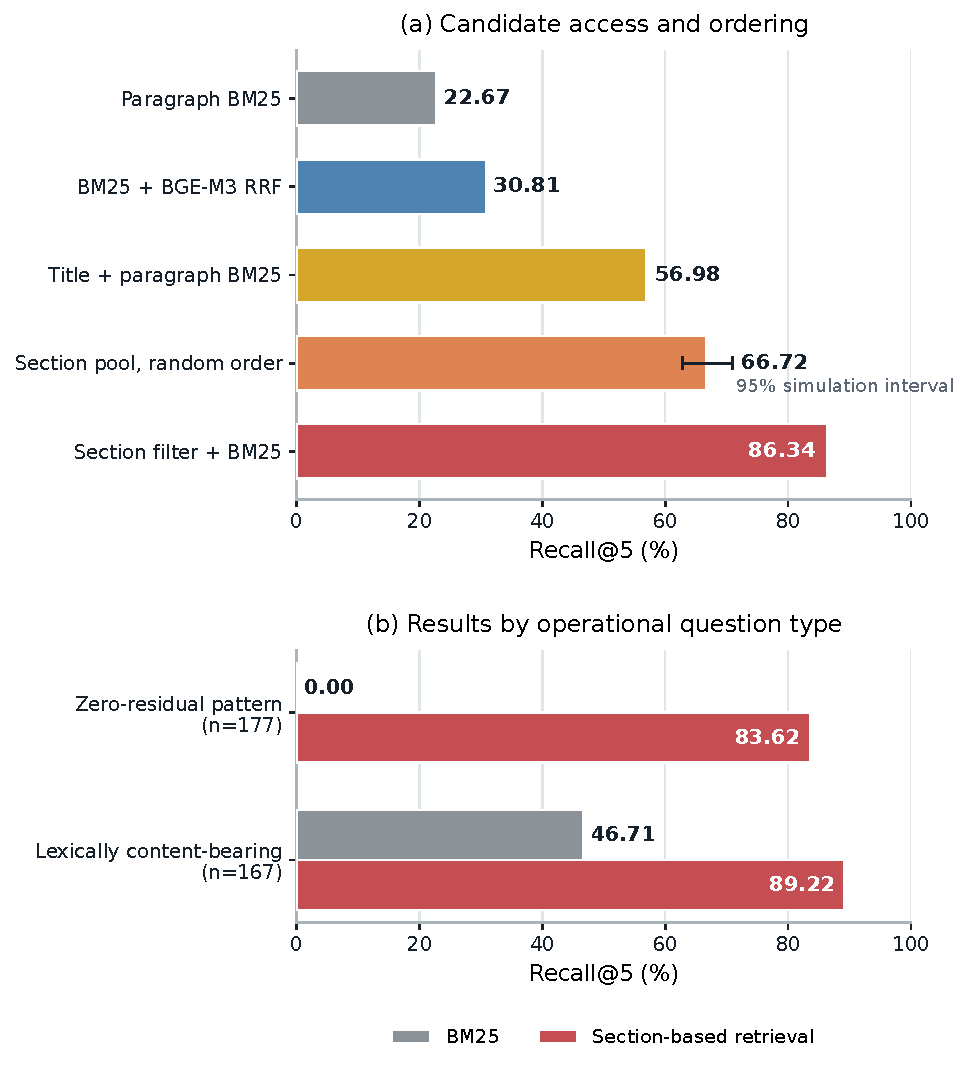
\includegraphics[width=\textwidth]{plots/21_retrieval_progression.pdf}
    \caption{Retrieval progression on the 344 test questions. Panel (a)
    compares content-based retrieval, title-aware BM25, random ordering after
    candidate reduction by section, and BM25 ranking within the same pool.
    Panel (b) compares paragraph BM25 and section-based retrieval across the
    two operational question groups. Panel (a) uses values from
    Tables~\ref{tab:dense_retrieval}, \ref{tab:modern_bge_indic}, and
    \ref{tab:metadata_controls}; panel (b) uses the question-group breakdown
    reported in Section~\ref{sec:citation_aware}.}
    \label{fig:retrieval_progression}
\end{figure}

\subsection{Candidate Ambiguity and Ranking Robustness}
\label{sec:candidate_ambiguity}

The section-filter system uses the first parsed section reference. Based on
this reference, 301 of the 325 parsed queries (92.6\%) match passages from
multiple Acts. The other 24 match passages from one Act.

A separate audit forms the union of candidates for every recognised section
reference in each question. Under this broader rule, 302 questions match
multiple Acts, 23 match one Act, and 19 have no recognised locator. The
one-question difference comes from a multi-reference Copyright question.
Its first locator, Section 30A, occurs in one Act, while its second locator,
Section 19, occurs in several Acts.

Section matching therefore narrows the candidate pool without necessarily
identifying the annotated Act. Retrieval evaluation measures agreement with
the annotated source; it does not establish that the system identified the
Act intended by the question. The separate human audit examines source
identifiability in 80 sampled cases with candidate evidence visible
(Section~\ref{sec:human_results}). It does not validate Act identification
across the full test set.

Section filtering reduces top-five annotated-source misses from 266 to 47
and cross-Act top-ranked mismatches from 188 to 40. Among the 40 misses for
parsed queries, 35 rank a passage from another Act first. Seven additional
misses use BM25 fallback. The remaining errors therefore mainly involve
provisions from different Acts that share a section number, although these
counts do not establish the reason for each error.

The broader all-reference grouping is a separate ambiguity audit. It measures
how many cross-Act alternatives are included when every recognised locator
in the question is considered. The reported section-filter outcomes use only
the system's first parsed locator. The union-based pool-size groups therefore
describe ambiguity but do not reproduce the exact candidate pools used during
inference.

Among the 302 multiple-Act questions, section-filter recall@5 is 100.00 for
pools of 2--5 passages, 91.28 for pools of 6--10, and 72.16 for pools of 11
or more. The corresponding reader F1 values are 78.26, 53.82, and 45.05.
The 23 one-Act questions reach 100.00 recall@5 and 88.57 reader F1. These
comparisons are descriptive because pool size is related to the Act and
question mix. The decline is concentrated in larger pools containing
provisions with the same section number from several Acts.

A separate tie-breaking check randomly orders passages with equal scores.
Across 10,000 random orders, mean recall@5 is 22.82 (SD 0.15) for BM25 and
86.30 (SD 0.18) for section filtering. The annotated paragraph is involved
in the rank-five boundary tie for only one BM25 query and two section-filter
queries.

\subsection{Full-Pipeline QA and Stage-by-Stage Errors}
\label{sec:section_end_to_end}

Higher retrieval recall does not necessarily lead to higher annotated-source
selection or answer scores under the fixed raw-logit decoder. To examine this
issue, each retrieval configuration passes its candidates to the fixed
\fixedreader{} reader and decoder described in
Section~\ref{sec:experimental_setup}. Retrieval and source selection do not
use the annotated paragraph identity.

\begin{table}[!htbp]
    \caption{Full-pipeline retrieval and extraction on the 344 test questions.
    ``Candidate-pool R@5'' is annotated-source recall before the active
    source-selection rule is applied. For the rank-1 condition, the reader
    receives only the passage selected by the BGE reranker. ``Selected source''
    is the percentage of cases in which the annotated paragraph is selected.
    Annotation-grounded F1 is zero when another paragraph is selected.
    All scores are on the 0--100 scale.}
    \label{tab:citation_aware_end_to_end}
    \centering
    \scriptsize
    \setlength{\tabcolsep}{3pt}
    \renewcommand{\arraystretch}{1.13}
    \begin{tabular}{@{}>{\raggedright\arraybackslash}p{4.4cm}rrrrr@{}}
        \toprule
        Setting & \shortstack{Candidate-pool\\R@5} &
        Selected source & EM & F1 &
        \shortstack{Annotation-\\grounded F1} \\
        \midrule
        Annotated paragraph + \fixedreader{} & 100.00 & 100.00 & 66.86 & 87.37 & 87.37 \\
        BM25 top-5 + \fixedreader{} & 22.67 & 11.92 & 10.47 & 31.95 & 11.08 \\
        Title+paragraph BM25 + \fixedreader{} & 56.98 & 30.52 & 23.55 & 45.07 & 27.85 \\
        Title-aware neural top-5 + \fixedreader{} & 83.72 & 37.79 & 30.23 & 53.12 & 35.41 \\
        Title-aware neural rank-1 + \fixedreader{} & 83.72 & 51.74 & 33.14 & 54.62 & 44.38 \\
        Section boost + \fixedreader{} & 86.34 & 45.35 & 36.34 & 55.22 & 42.72 \\
        Section filter + \fixedreader{} & 86.34 & 50.87 & 38.37 & 57.99 & 47.29 \\
        Section filter + BGE selector + \fixedreader{} & 86.34 & 56.40 & 35.76 & 58.47 & 48.62 \\
        \bottomrule
    \end{tabular}
    \begin{flushleft}
        {\scriptsize The annotated-paragraph row is an upper-bound reading
        condition, not a full-pipeline system. The two title-aware neural rows
        use the title-plus-paragraph RRF pool reranked by BGE. In the top-5
        row, raw reader logits select among five passages. In the rank-1 row,
        the BGE reranker selects the first passage and the reader extracts
        from it. In the final row, BGE-reranker-v2-m3 selects a passage from
        the unchanged section-filter top-five pool using the question and
        title-plus-paragraph text. The fixed reader then extracts from that
        single passage. The 19 unparsed queries use the documented BM25
        fallback.}
    \end{flushleft}
\end{table}
\FloatBarrier

Title-plus-paragraph BM25 reaches 45.07 F1, while section filtering reaches
57.99. This is a difference of 12.92 points over the metadata-matched
baseline (Table~\ref{tab:citation_aware_end_to_end}). A paired bootstrap over
source clusters gives a 95\% interval of $[6.62,19.44]$ for this difference
(75 Act--section clusters, 10,000 resamples, seed 42).

Compared with paragraph-only BM25, filtering and boosting increase F1 by
26.03 and 23.26 points, respectively. Their source-cluster bootstrap
intervals are $[19.01,33.00]$ and $[16.31,30.13]$.

The strongest title-aware neural retriever closes much of the retrieval gap.
Its annotated-source recall@5 is 83.72, compared with 86.34 for section
filtering. When raw reader logits select among its top five passages,
annotated-source selection is 37.79, F1 is 53.12, and annotation-grounded F1
is 35.41. When the BGE rank-one passage is used instead, these values rise
to 51.74, 54.62, and 44.38, respectively.

For section filtering, the corresponding values are 50.87, 57.99, and 47.29
with reader-based source selection. With the independent BGE selector, they
are 56.40, 58.47, and 48.62. Adding titles therefore makes the neural
retrieval comparison much stronger, but the candidate pool and
source-selection rule still affect final answer scores.

The section-filter pipeline with BGE selection achieves 3.85 more F1 points
than the title-aware neural rank-one pipeline. A paired bootstrap over the
same 75 Act--section source clusters gives a 95\% interval of
$[-0.16,8.73]$ (10,000 resamples, seed 42). Because this interval includes
zero, this post-hoc comparison does not show a clear F1 difference between
the two pipelines.

Although boosting and filtering have the same recall@5, filtering achieves
higher F1, at 57.99 versus 55.22, and higher annotated-source selection, at
50.87 versus 45.35. Filtering removes nonmatching sections before reader
scoring. It raises F1 from 17.59 to 58.43 for the zero-residual group and
from 47.17 to 57.52 for the lexically content-bearing group.

The independent BGE selector tests whether the remaining source-selection
errors are caused only by comparing raw reader span logits across passages.
It increases annotated-source selection from 50.87 to 56.40 and conditional
source selection from 58.92 to 65.32, while F1 changes from 57.99 to 58.47.
The alternative selector therefore improves annotation-relative source
selection but still chooses another paragraph in 103 of the 297 cases where
the annotated paragraph is available. This check reduces dependence on the
main decoder rule. However, the selector remains zero-shot and is evaluated
against annotation identity rather than expert legal relevance.

Table~\ref{tab:stage_decomposition} further separates the remaining errors.

\begin{table}[!htbp]
    \caption{Stage-by-stage outcomes for the 344 test questions. The four
    outcome columns are separate counts. ``Avail., other'' means that the
    annotated source is available but the source-selection rule chooses
    another source. ``Source, not exact'' and ``Source, exact'' mean that the
    rule chooses the annotated source without or with an exact answer match.
    ``Conditional source'' is the percentage of available annotated
    paragraphs selected by the active source-selection rule.
    Annotation-grounded F1 is on the 0--100 scale.}
    \label{tab:stage_decomposition}
    \centering
    \scriptsize
    \setlength{\tabcolsep}{3pt}
    \begin{tabular}{@{}lrrrrrr@{}}
        \toprule
        Setting & \shortstack{Source\\absent} &
        \shortstack{Avail.,\\other} &
        \shortstack{Source,\\not exact} &
        \shortstack{Source,\\exact} &
        \shortstack{Cond.\\source (\%)} &
        \shortstack{Grounded\\F1} \\
        \midrule
        BM25 & 266 & 37 & 8 & 33 & 52.56 & 11.08 \\
        Title+paragraph BM25 & 148 & 91 & 28 & 77 & 53.57 & 27.85 \\
        Title-aware neural top-5 & 56 & 158 & 30 & 100 & 45.14 & 35.41 \\
        Title-aware neural rank-1 & 56 & 110 & 64 & 114 & 61.81 & 44.38 \\
        Section boost & 47 & 141 & 33 & 123 & 52.53 & 42.72 \\
        Section filter & 47 & 122 & 44 & 131 & 58.92 & 47.29 \\
        Section filter + BGE selector & 47 & 103 & 71 & 123 & 65.32 & 48.62 \\
        \bottomrule
    \end{tabular}
\end{table}
\FloatBarrier

Figure~\ref{fig:stage_decomposition} shows the four outcomes. With section
filtering, the annotated source is absent in 47 cases, available but not
selected in 122, selected without an exact answer match in 44, and selected
with an exact match in 131. Raw F1 is 57.99, compared with
annotation-grounded F1 of 47.29. This difference shows that answers from
other sources can receive token-overlap credit. Decoder alternatives retain
this failure category (Appendix~\ref{app:review_checks}).

The independent BGE selector changes these counts to 47, 103, 71, and 123.
Although it selects the annotated source more often, it does not produce more
exact matches because the fixed reader predicts a non-exact span in more of
the additionally selected annotated paragraphs. The title-aware neural
top-five condition has counts of 56, 158, 30, and 100. Direct BGE rank-one
selection changes them to 56, 110, 64, and 114.

\begin{figure}[!htbp]
    \centering
    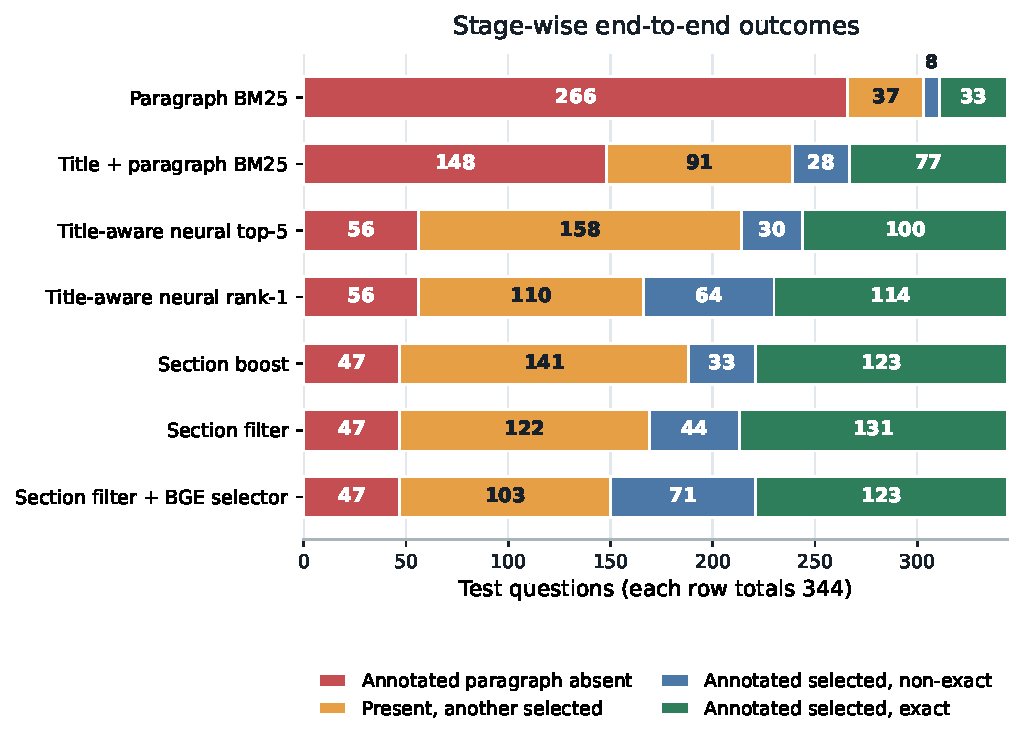
\includegraphics[width=\textwidth]{plots/22_stagewise_outcomes.pdf}
    \caption{Stage-by-stage outcomes for seven pipelines using the same fixed
    answer reader on the 344 test questions. The rank-one and selector rows
    use the independent BGE reranker for source selection. Direct labels show
    question counts, and each row totals 344. ``Exact'' denotes normalised
    exact match. Section filtering greatly reduces the number of cases in
    which the annotated paragraph is absent from the top five, but
    source-selection errors remain substantial.}
    \label{fig:stage_decomposition}
\end{figure}

For the 325 questions with a parsed section reference, BM25 and section
boosting reach recall@5 of 20.31 and 87.69, respectively. For the 19 questions
without a parsed section reference, both reach 63.16 through the same BM25
fallback. This subgroup is too small to characterise retrieval for questions
without parsable statutory locators.

\section{Reference Sensitivity and Redirection Stress Tests}
\label{sec:citation_ablation}

Four query variants examine the role of statutory references in retrieval:
the original query, a query with the reference removed, a reference-only
query, and a query in which the first section number is replaced with another
section number from the same Act. Reference removal includes minor wording
cleanup. The reference-only query keeps the first section locator and removes
the other wording. The replacement query keeps the remaining wording
unchanged. It is an artificial redirection stress test, not a model of user
error. The annotated Act is used only to select the replacement section; it
is not provided to the retriever.

Replacement sections are sampled uniformly from other sections in the
annotated Act. Keeping the original clause wording can make the modified query
inconsistent. Recall remains measured against the original annotated
paragraph. The experiment uses random seeds 7, 42, and 99.
Table~\ref{tab:citation_ablation} reports the results for seed 42.

Of the 344 test questions, 325 contain a parsed section reference. The other
19 questions receive neither a reference-only nor a replacement variant,
although the wording-cleanup procedure changes six of them. No models are
retrained. This experiment uses a 384-token cross-encoder limit rather than
the 512-token limit used in the main reranking comparison. Its original-query
scores are therefore specific to this experimental setting.

The section-boost system follows the 1,000-point rule defined in
Section~\ref{sec:citation_aware}. Removing the reference causes this system
to use unrestricted BM25 because no section can receive the boost. Replacing
the section number changes which passages receive the boost by construction.
The content-based retrieval systems provide comparisons in which this
redirection is not explicitly programmed.

\begin{table}[!htbp]
    \caption{Recall@5 under statutory-reference interventions for
    representative systems. Removal includes minor wording cleanup.
    Replacement leaves the other wording unchanged. Reference only retains
    the first section reference. Section boost uses the deterministic
    1,000-point rule. Questions without a parsed reference have no
    reference-only or corrupted-reference variant. All values are
    percentages; corrupted-reference values use seed 42.}
    \label{tab:citation_ablation}
    \centering
    \small
    \setlength{\tabcolsep}{4pt}
    \begin{tabular}{@{}llrrrr@{}}
        \toprule
        Group & System & Original & Ref.\ removed & Ref.\ only &
        Corrupted ref. \\
        \midrule
        \multicolumn{6}{@{}l}{\textit{Zero-residual pattern ($n=177$)}} \\
        & BM25                 &  0.00 &  1.13 &  0.00 &  0.56 \\
        & Hybrid + CE          &  0.56 &  0.00 &  0.00 &  1.69 \\
        & Section boost + BM25 & 83.62 &  1.13 & 62.71 &  0.00 \\
        \midrule
        \multicolumn{6}{@{}l}{\textit{Lexically content-bearing, with
        parsed references ($n=148$)}} \\
        & BM25                 & 44.59 & 42.57 &  2.03 & 43.92 \\
        & Hybrid + CE          & 60.14 & 54.05 & 10.14 & 49.32 \\
        & Section boost + BM25 & 92.57 & 42.57 & 65.54 & 11.49 \\
        \midrule
        \multicolumn{6}{@{}l}{\textit{Control without parsed references
        ($n=19$)}} \\
        & BM25                 & 63.16 & 63.16 & --- & --- \\
        & Section boost + BM25 & 63.16 & 63.16 & --- & --- \\
        \bottomrule
    \end{tabular}
    \begin{flushleft}
        {\scriptsize Corrupted-reference recall@5, reported as mean
        $\pm$ standard deviation over the three corruption seeds, is
        $0.00\pm0.00$ for section boosting on zero-residual questions and
        $12.61\pm1.03$ for section boosting on lexically content-bearing
        questions with parsed references.}
    \end{flushleft}
\end{table}

\begin{figure}[!htbp]
    \centering
    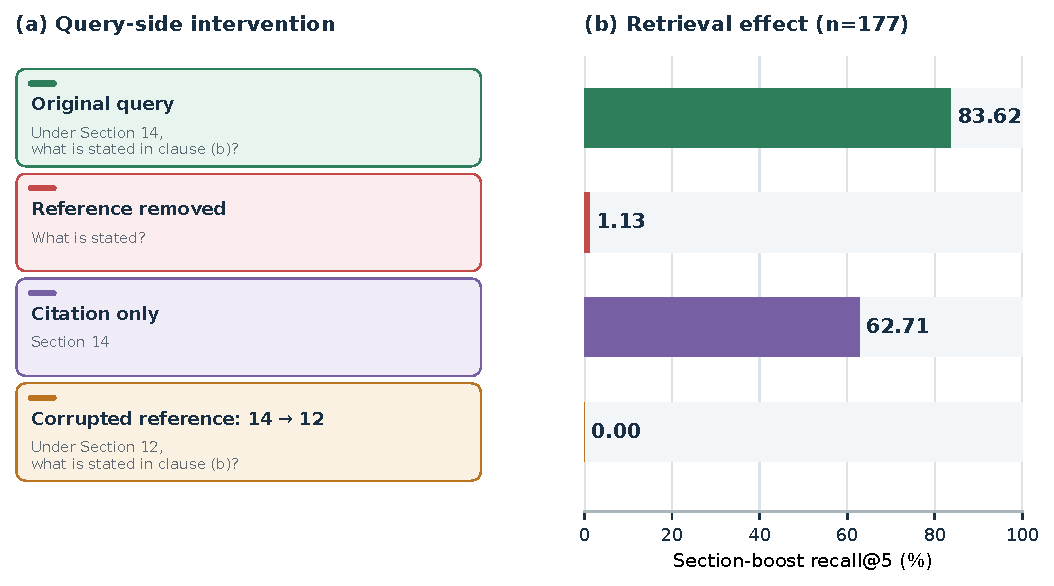
\includegraphics[width=\textwidth]{plots/23_citation_intervention.pdf}
    \caption{Query-reference intervention on the 177 zero-residual questions.
    Panel (a) shows an actual Copyright Act question and its saved
    transformations under seed 42. Panel (b) reports aggregate section-boost
    recall@5 across all 177 questions, measured against the original annotated
    paragraphs. The values do not refer only to the example in panel (a).
    Reference removal includes minor wording cleanup. Reference only retains
    the first section reference. The corrupted-reference condition uses
    another valid section from the same Act. It is a stress test, not an
    answer-preserving rewrite.}
    \label{fig:citation_intervention}
\end{figure}

For the 177 zero-residual questions, removing the reference reduces
section-boost recall@5 from 83.62 to 1.13. Replacing the section number reduces
recall@5 to 0.00 under all three seeds. Reference-only queries retain 62.71
recall@5 (Table~\ref{tab:citation_ablation};
Figure~\ref{fig:citation_intervention}). These interventions are exploratory
because they reuse the test set and were not preregistered.

For the 148 lexically content-bearing questions with parsed references,
section-boost recall@5 falls from 92.57 to 42.57 after reference removal and
to 11.49 after replacement under seed 42. For Hybrid+CE, reference replacement
reduces recall@5 from 60.14 to 49.32. The smaller removal effect in this group
is consistent with descriptive wording partly compensating for the missing
reference. For the 19 questions without parsed references, BM25 and section
boost both reach 63.16 recall@5 through the same unrestricted-BM25 fallback.

The decline under section boosting after reference replacement is expected
because the system assigns its score bonus to the substituted section
identifier. This result confirms the direction of the programmed redirection;
it does not show a learned failure mechanism. The change under Hybrid+CE is
a more informative non-programmed comparison because that pipeline does not
use a section-matching rule. However, the effect is smaller and remains
specific to these artificial query modifications.

In the section-based system, statutory references direct retrieval toward
passages with matching section identifiers. The remaining query wording then
helps BM25 rank passages that share the matched identifier. Artificially
replacing a reference can redirect retrieval away from the annotated
paragraph. Even when the annotated paragraph is retrieved, source selection
and answer extraction remain separate stages of the pipeline.


%% ============================================================
\section{Human Evaluation of Sources and Answers}
\label{sec:human_results}

Automatic evaluation measures annotated-source recovery and selection,
together with EM and token-level F1 against the annotated answer. The human
audit separately examines the assessed legal adequacy of the supplied sources
and answers. It does not replace the benchmark annotations or change the
reported EM, F1, or retrieval recall scores.

The original separate ratings show 90.00\% agreement on selected-source
relevance ($\kappa=0.755$, AC1 $=0.884$, $n=80$) and 79.75\% agreement on
predicted-answer correctness ($\kappa=0.655$, AC1 $=0.749$, $n=79$).
Agreement on whether the question uniquely identifies the annotated source
is lower, at 62.03\% ($\kappa=0.199$, AC1 $=0.502$, $n=79$). For the selected
source, the corresponding values are 63.29\%, $\kappa=0.304$, and
AC1 $=0.516$ ($n=79$). Agreement between the two reviewers therefore varies
across the assessment criteria. However, low agreement on source uniqueness
alone does not establish that a question is ambiguous.

\begin{table}[!htbp]
    \caption{Final consensus judgements by section-filter pipeline outcome.
    Each row contains 20 audited questions; $N$ is the size of the
    corresponding group in the full test set. Relevance counts only
    ``Yes.'' Predicted-answer correctness retains all four categories.
    Materiality counts ``Moderate'' or ``High.'' It is a separate judgement,
    not a transformation of correctness or token overlap.}
    \label{tab:human_consensus}
    \centering
    \scriptsize
    \setlength{\tabcolsep}{4pt}
    \begin{tabular}{@{}>{\raggedright\arraybackslash}p{3.6cm}
        rr@{\hspace{9pt}}rrrrr@{}}
        \toprule
        & & \shortstack{Selected source\\relevant}
        & \multicolumn{4}{c}{Predicted answer correct}
        & \shortstack{Moderate/\\high error} \\
        \cmidrule(lr){4-7}
        Pipeline outcome & $N$ & Yes & Yes & Partly & No & Unclear & \\
        \midrule
        Annotated source absent       & 47  & 8  & 7  & 2 & 7 & 4 & 9  \\
        Available, other selected     & 122 & 11 & 10 & 1 & 9 & 0 & 10 \\
        Selected, non-exact           & 44  & 18 & 9  & 8 & 3 & 0 & 11 \\
        Selected, exact answer        & 131 & 17 & 16 & 0 & 3 & 1 & 3  \\
        \bottomrule
    \end{tabular}
\end{table}

Table~\ref{tab:human_consensus} shows that matching the annotated source and
assessed legal adequacy are different measures. Among the 40 audited cases in
which the system selected another source, the final consensus ratings
classified 17 predicted answers as correct, three as partly correct, 16 as
incorrect, and four as unclear. However, none of the selected and annotated
source pairs was judged fully equivalent: 39 were classified as
non-equivalent and one as partly equivalent.

The written reasons for answers rated correct often described questions that
did not specify an Act. In these cases, the reviewers considered an answer
from another selected provision correct under a different plausible
interpretation. This assessment does not establish that the selected source
governs the legal question intended by the benchmark. Among the same 40
cases, 19 received moderate or high error-materiality ratings. Under the
audit criteria, these errors include missing information or incorrect answers
that affect the legal meaning of the response. These findings describe the
audited cases and do not estimate legal error rates across all
annotated-source retrieval failures.

An exact match with the annotated answer also does not guarantee assessed
legal adequacy. Among the 20 audited cases in which the annotated source was
selected and the answer matched exactly, the final consensus ratings
classified 16 answers as correct, three as incorrect, and one as unclear.
The three answers rated incorrect involved text assigned across a section
boundary, an extracted cross-reference fragment, or material from a schedule
assigned to the wrong section. The unclear case concerned a problem with the
question wording. These assessments concern the retained benchmark evidence;
they do not represent corrected benchmark annotations.

Among the 20 cases in which the annotated source was selected but the answer
did not match exactly, nine answers were judged correct, eight partly correct,
and three incorrect. The written reasons distinguish minor differences in
answer length from errors involving missing conditions or exceptions.

These findings show that neither exact answer matching nor annotated-source
matching fully agrees with the human assessments in this sample. The
assessments concern legal adequacy relative to the archived evidence supplied
to the reviewers. They do not independently identify the governing legal
provision, verify the current state of the law, or establish the legal
accuracy of the complete benchmark.

\FloatBarrier

\section{External Retrieval Comparison on UK-StatuteCorpus}
\label{sec:uk_external_validation}

This experiment provides an external comparison of content retrieval outside
the Indian benchmark. It evaluates the original small-model systems and the
modern BGE extension on UK-StatuteCorpus Eval100
\citep{alshehri2026neural}. The dataset contains 100 English questions over
124,796 UK statutory passages from 2020--2024. Each question has three
relevant passages, one at each relevance grade from 1 to 3. This gives 300
graded relevance judgements.

UK-StatuteCorpus provides passage-level relevance labels rather than answer
spans. This experiment therefore evaluates retrieval ranking only. It does
not repeat the retrieval--reading, source-selection, or answer-extraction
analysis used for IndicIPR-QA.

The saved run record contains the corpus, query, model, and evaluation
settings. The UK experiments use depth-100 retrieval and fusion rankings,
followed by reranking of the first 50 candidates. The legacy cross-encoder,
BGE-M3, and BGE-reranker-v2-m3 use a maximum sequence length of 512 tokens.
The BGE extension uses paragraph text only and the same pinned model revisions
as the Indian comparison in Table~\ref{tab:modern_bge_indic}.

The UK queries are not processed using the Indian section parser or the
reference-removal, reference-only, and corrupted-reference transformations.
Only the fixed system preprocessing is applied. This includes trimming query
strings, using lowercase alphanumeric tokenisation for BM25, and applying
the standard ``query:'' and ``passage:'' prefixes for E5. The BGE systems
use the archived settings recorded for the experiment. No Act names or
section titles are added. A separate UK reference audit records reference
patterns but does not modify the evaluated queries.

For the UK evaluation, let \(G_i\) be the set of all released passages with
positive relevance for query \(i\), and let \(T_{ik}\) be the top \(k\)
retrieved passages. Recall is the mean of the recall values for the individual
questions:
\[
\mathrm{R@}k
=\frac{100}{n}\sum_{i=1}^{n}
\frac{|T_{ik}\cap G_i|}{|G_i|},
\qquad n=100.
\]
The leading factor converts the result to a percentage. This measure is not
a pooled count or the percentage of questions with at least one relevant
passage retrieved. Grade-3 recall uses only the passage with relevance grade
3 for each query. nDCG@10 uses all released relevance grades with the gain
function \(2^{\mathrm{rel}}-1\).

IndicIPR-QA has one annotated paragraph per question, so its recall measures
whether that paragraph is retrieved. Recall therefore has different meanings
in the two benchmarks. Table~\ref{tab:uk_external_retrieval} reports the UK
retrieval results.

\begin{table}[!htbp]
    \caption{External retrieval comparison on UK-StatuteCorpus Eval100
    (100 questions). Recall uses all released relevant passages. Grade-3
    R@10 uses only the highest-relevance judgement for each question.}
    \label{tab:uk_external_retrieval}
    \centering
    \scriptsize
    \setlength{\tabcolsep}{2.3pt}
    \begin{tabular}{@{}lrrrrrr@{}}
        \toprule
        System & R@5 & R@10 & R@50 & MRR@10 & nDCG@10 & G3 R@10 \\
        \midrule
        BM25
        & 25.67 & 33.67 & 52.67 & 40.83 & 27.13 & 45.00 \\
        E5-small-v2
        & 20.67 & 31.67 & 52.67 & 33.54 & 28.27 & 53.00 \\
        BM25 + E5 RRF
        & 27.33 & 40.33 & 55.67 & 43.61 & 33.61 & 60.00 \\
        BM25 + legacy cross-encoder
        & 27.33 & 37.33 & 52.67 & 44.18 & 33.66 & 57.00 \\
        BM25--E5 RRF + legacy cross-encoder
        & 25.67 & 36.67 & 55.67 & 43.49 & 33.27 & 56.00 \\
        \midrule
        BGE-M3
        & 29.33 & 42.00 & 57.00 & 49.13 & 37.45 & 62.00 \\
        BM25 + BGE-M3 RRF
        & 31.33 & 40.67 & 59.33 & 47.32 & 34.21 & 61.00 \\
        BM25 + BGE reranker
        & 30.67 & 40.67 & 52.67 & 55.87 & 38.32 & 61.00 \\
        BM25--BGE-M3 RRF + BGE reranker
        & 32.00 & 43.33 & 59.33 & 56.81 & 40.53 & 67.00 \\
        \bottomrule
    \end{tabular}
    \begin{flushleft}
        {\scriptsize All scores are on the 0--100 scale. The
        machine-readable summary reports proportions and bootstrap
        intervals.}
    \end{flushleft}
\end{table}

Table~\ref{tab:uk_external_retrieval} shows that the modern models provide a
stronger content-retrieval comparison. BGE-M3 raises recall@10 from 33.67
for BM25 to 42.00, a gain of 8.33 points. A paired bootstrap over questions
gives a 95\% interval of $[2.67,14.00]$ for this difference. BGE-M3 also
raises nDCG@10 by 10.32 points, with a 95\% interval of
$[4.23,16.23]$.

BM25--BGE-M3 fusion gives the highest initial-retrieval recall@5, at 31.33,
and has a recall@50 ceiling of 59.33. Applying the BGE reranker to this
candidate pool produces the highest MRR@10, nDCG@10, and Grade-3 recall@10
in the table, at 56.81, 40.53, and 67.00, respectively.

Compared with BGE fusion before reranking, the BGE reranker raises nDCG@10
by 6.32 points, with a 95\% interval of $[2.22,10.54]$. However, recall@5
increases by only 0.67 points, and its interval includes zero:
$[-3.33,4.67]$. The reranker therefore produces a clear gain in nDCG@10 in
this comparison, but not a clear gain in recall@5.

All intervals use 10,000 paired bootstrap resamples at the question level
with seed 42. On Eval100, dense retrieval, fusion, and reranking improve
different retrieval metrics. The reference-subgroup audit is reported in
Appendix~\ref{app:uk_reference}. Because the datasets, relevance labels, and
evaluation measures differ, this experiment is an additional comparison of
content retrieval. It is not a replication of the Indian section-filtering,
source-selection, or answer-extraction analysis.

\FloatBarrier

\section{Discussion}
\label{sec:discussion}

This study examines annotated-source retrieval, source selection, and answer
extraction as separate stages. Section filtering achieves high retrieval
scores on this reference-heavy benchmark. The title-aware BGE reranking
pipeline reduces the recall@5 difference with section filtering to 2.62
points. This result shows that the tested neural pipeline can use section
titles when they are provided.

However, improved retrieval does not remove source-selection errors. Section
filtering retrieves the annotated source in its top five candidates for
86.34\% of the questions, but the fixed reader decoder selects it in only
50.87\%. An independent BGE selector raises annotated-source selection to
56.40\%. Source-selection errors therefore remain when raw reader logits are
replaced by an independent reranker, although other selection methods may
produce different results.

The UK comparison shows that dense retrieval, fusion, and reranking improve
different retrieval metrics on UK-StatuteCorpus Eval100. However, it evaluates
content retrieval only. It does not validate the Indian section-filtering,
source-selection, or answer-extraction results in another jurisdiction.

\subsection{What Does the Benchmark Measure?}

Gold-context F1 measures answer extraction when the annotated paragraph is
provided. It does not measure retrieval, source selection, or open legal
research. A reference such as ``Section 25'' may help locate information
within a supplied paragraph, but the same section number can occur in several
Acts.

The operational question grouping helps examine this difference.
Appendix~\ref{sec:classifier_robustness} reports results under different token
thresholds. The groups are defined by a text rule rather than expert
judgements about question meaning. Because the questions were generated and
then curated, the groups may not represent the types of questions asked by
legal practitioners. Section~\ref{sec:limitations} discusses this limitation
further.

Full-pipeline F1 can also give token-overlap credit to an answer extracted
from a non-annotated source. Annotation-grounded F1 and source-selection
counts therefore provide information that raw EM and F1 do not show.

The final human assessments rated some answers from non-annotated sources as
correct and some exact matches as incorrect. Agreement with benchmark
annotations therefore does not always match assessed legal adequacy. The
reviewers also had lower agreement on source uniqueness than on several other
assessment criteria. This uncertainty limits conclusions about source
uniqueness beyond the audited sample.

\subsection{Implications for Legal Information Access}

A statutory reference identifies a provision within a legal structure. Its
interpretation depends on the Act and its organisation
\citep{louisFindingLaw2023,noceJuriFindITItalian2026}. Because the same
section number can occur in different Acts, matching a section identifier
alone may not identify the intended source.

Table~\ref{tab:qualitative} gives an example in which the BM25--reader
pipeline answers a Trade Marks Act question using a passage from the Patents
Act. This is a mismatch with the benchmark annotation. It does not establish
which provision legally governs the question. Displaying the Act name,
section, and source passage alongside the answer could make this type of
source mismatch visible to users.

\subsection{Legal Significance of Retrieval Errors}

Provisions with similar wording may differ in their scope, conditions, or
exceptions. A source that differs from the benchmark annotation may therefore
change the legal meaning of an answer. However, an annotation mismatch alone
does not prove that the selected source or answer is legally incorrect.

This study does not assess harm caused by legal advice or determine which
provision governs a particular legal question. The human audit is limited to
the questions, statutory passages, and answers supplied to the reviewers. It
shows why answer overlap, source identity, legal relevance, and assessed error
materiality should be considered together when interpreting the sampled
outcomes. It does not verify the current state of the law or estimate legal
error rates across the full test set.

\subsection{Implications for Statutory QA System Design}

The metadata controls show that passage representation affects recovery of
the annotated source on this benchmark. Paragraph text alone excludes useful
title information. Adding section titles improves retrieval with both BM25
and the tested neural pipeline. Section filtering narrows the candidate pool,
while BM25 ranking within the section-matched pool improves recovery compared
with random ordering.

These findings do not establish that strong retrievers are generally unable
to use statutory structure. Instead, they support further testing of richer
metadata, including Act, section, subsection, and clause hierarchies,
relationships between provisions, and cross-references. The additional value
of these features was not tested in this study.

For systems handling questions similar to those in this benchmark, matching
query locators with statutory metadata may help identify relevant candidates.
Content-based ranking can then distinguish passages that share the same
section number. A fallback retrieval method can handle questions without a
parsed section reference.

A system could also compare the selected source with the reference and
descriptive wording in the question. Such a check may identify some retrieval
redirections. However, questions that do not contain enough information may
remain difficult to resolve. Clause-level matching and cross-reference parsing
were not evaluated in this study.

\subsection{Implications for Benchmark Design}

For benchmarks containing similar question patterns, separate reporting for
zero-residual reference-pattern and lexically content-bearing questions may
make aggregate results easier to interpret. Benchmarks could also report
candidate access, source selection, and answer extraction separately.

Separate evaluation tracks could test locator resolution, content retrieval,
source selection, and answer extraction from an identified provision. Human
assessment can then examine whether annotation agreement corresponds to
assessed legal adequacy without treating the two measures as equivalent.

\section{Limitations}
\label{sec:limitations}

The findings apply mainly to this benchmark and its evaluation setting.
Retrieval from paragraph text alone excludes section identifiers and headings
from passage titles, although many generated questions refer to this
information. Part of the retrieval difficulty therefore comes from
information missing from the indexed representation. Adding section titles
to the neural pipeline reduces the recall@5 difference between BGE reranking
and section filtering to 2.62 points. However, full-pipeline performance still
depends on the source-selection rule.

The neural retrievers and rerankers are used without legal-retrieval
fine-tuning. This limitation does not apply to the fixed reader, which was
fine-tuned on the IndicIPR-QA training split. The experiments evaluate selected
model configurations and do not provide a comprehensive comparison of
title-aware retrievers.

The operational question grouping and section parser have not been validated
through human judgements of question meaning. The questions were generated
and then curated, so the frequency of explicit statutory references may
differ from naturally occurring legal questions. Repeated question patterns
may also make section references especially useful. The results may therefore
partly reflect how the questions were generated and filtered rather than how
users normally ask legal questions. Comparisons within Acts do not fully
separate these effects. Evaluation on independently written,
practitioner-generated questions, with and without explicit references,
remains an important direction for future work. No such question set is
evaluated here.

The reader's raw span scores are not calibrated across passages. The results
therefore depend on both the retrieved candidates and the fixed
source-selection rule. They do not provide an upper bound on
source-selection performance. Passages divided into more input windows also
have more opportunities to receive a high raw score. The independent
BGE-based selector improves annotated-source selection, but this does not
establish that its scores are calibrated or that its selected sources are
legally relevant. It remains a zero-shot selector evaluated against annotation
identity.

The remaining words in a question may reflect legal content, statutory
headings, or the style of the question generator. Equal retrieval scores and
corpus ordering may also affect ranking, although the tie-sensitivity checks
show limited effects in the tested runs. The original dataset validation
covers 200 question--answer pairs \citep{anonymous2026indiciprqa}. The
separate 80-case human audit in this study examines outputs from the
section-filter pipeline and their retained benchmark annotations.

The human audit involves two law graduate students and 20 cases sampled from
each of four pipeline outcomes. It is not a practitioner study or an
independent third-party legal adjudication. The source-identifiability results
reported here were judged with two candidate passages visible. They therefore
do not establish whether the question alone identifies a unique source across
the full statutory corpus.

Agreement varies across the assessment fields, especially source uniqueness
and text quality. During consensus discussion, the reviewers could revise
labels on which they had originally agreed as well as labels on which they
had disagreed. The final consensus ratings do not constitute an independent
legal standard.

The audit uses a balanced stratified sample rather than a sample proportional
to the four pipeline-outcome populations. Therefore, the unweighted pooled
results do not estimate population-level legal error rates for all 344 test
questions. The audit also does not validate the operational question grouping
or section parser, compare legal adequacy across retrieval systems, correct
the benchmark annotations, or independently replicate the retrieval study.
A larger follow-up should include practising lawyers or legal researchers,
independent adjudication, and a sampling design that supports population-level
estimates.

The same 344 test questions support reader selection, diagnosis, and
evaluation. The fixed reader was selected from earlier configurations after
results were available, and the study records do not contain a complete list
of the alternatives considered. The operational grouping used in RQ2 was
developed after examining the test material. The query interventions were
defined before their experimental runs but were not preregistered. These
analyses therefore describe a fixed benchmark; they do not confirm a general
relationship on unseen questions.

The evaluated retrieval methods include BM25, four small zero-shot dense
encoders, BGE-M3, two cross-encoders, retrieval fusion, and a rule-based
section-reference procedure. The BGE extension provides a stronger
general-purpose comparison but is not a legally supervised retriever. The
experiments do not evaluate supervised legal retrievers, late-interaction
models, alternative title-aware neural architectures, or finer-grained
matching at the clause level. Recall@50 limits the annotated sources that a
reranker can recover from its initial candidate pool. The near-zero results
for zero-residual questions also limit conclusions about the tested learned
systems.

Training retrievers on statutory question--provision pairs is an important
next comparison. Supervised retrievers, LLM-based rerankers, or generative QA
pipelines may achieve higher performance. Evaluating these methods would move
the study towards system improvement rather than diagnosis alone. The purpose
of the present study is to identify errors in retrieval and source selection,
not to claim that the evaluated systems are the best available methods.

The UK experiment evaluates content retrieval but does not reproduce the full
diagnostic analysis conducted on IndicIPR-QA. In addition, only 19
IndicIPR-QA questions have no parsed statutory reference. A closer external
replication would require aligned provision-level relevance judgements, answer
evidence, suitable models, and overlapping statutory locators.
UK-StatuteCorpus, EQUALS, BSARD, JuriFindIT, and IL-TUR do not provide all
these conditions in one aligned setting
\citep{chen2023equals,louisSpanakisBSARD2022,noceJuriFindITItalian2026,
joshiILTUR2024}.

IndicIPR-QA is limited to answerable English questions with one annotated
source paragraph, drawn from seven Indian intellectual property Acts. The
findings do not establish transfer to other jurisdictions or legal fields,
case law, contracts, or multilingual systems. The benchmark does not evaluate
unanswerable questions, questions requiring evidence from multiple sections,
or interactive settings.

Future research should apply the diagnostic framework to LLM and RAG
pipelines, independently written questions, and legal documents from other
fields, jurisdictions, and languages. The current legal status and
consolidation of the archived statutes have not been independently verified.
The findings should not be interpreted as legal advice.

\FloatBarrier


% Keep the short conclusion together without changing font size or margins.
\begin{samepage}
\section{Conclusion}
\label{sec:conclusion}

This study examines where errors arise when a statutory QA pipeline must retrieve and select evidence before extracting an answer with a fixed reader. On IndicIPR-QA, F1 falls from 87.37 with the annotated paragraph to 31.95 when BM25 retrieves the top five candidates from paragraph text alone. Adding section titles or matching section identifiers improves recovery of the annotated source, showing that passage representation matters alongside retrieval model choice. However, the same section number can occur in different Acts. Under section filtering, the annotated source appears in the top five for 86.34\% of the questions, but the fixed reader decoder selects it in only 50.87\%. An independent BGE selector raises annotated-source selection to 56.40\%, but source-selection errors remain. The human audit further shows that agreement with benchmark annotations and assessed legal adequacy can differ in the sampled cases. These findings are specific to the evaluated benchmark, systems, and audit sample. Section filtering is a diagnostic intervention, and the zero-residual question-pattern analysis is exploratory. Reporting annotated-source retrieval, source selection, and answer extraction separately helps explain the aggregate QA score in this setting. Validation with independently written questions and questions requiring evidence from multiple sections remains an important direction for future work.
\end{samepage}

\clearpage

%% ============================================================

\appendix
\section{Retrieval Diagnostics and Robustness Audits}
\label{app:secondary}

This appendix documents the sources of the data, models, and analyses used in
the study. It also reports robustness checks for the question grouping rule,
results across Acts, and qualitative retrieval cases.

\subsection{Sources of Data, Models, and Analyses}

Table~\ref{tab:analysis_provenance} separates the inherited dataset and fixed
reader from the analyses conducted in this study. \fixedreader{} is the
LEGAL-BERT-BASE checkpoint trained first on SQuAD-v1 and then on IndicIPR-QA.
The checkpoint was selected after earlier results were available and remains
fixed throughout these experiments. It is not a new model architecture.

\begin{table}[!htbp]
    \caption{Provenance of the datasets, models, and analyses used in this
    study.}
    \label{tab:analysis_provenance}
    \centering
    \scriptsize
    \setlength{\tabcolsep}{3.5pt}
    \renewcommand{\arraystretch}{1.20}
    \begin{tabular}{@{}
        >{\raggedright\arraybackslash}p{4.0cm}
        >{\raggedright\arraybackslash}p{2.0cm}
        >{\raggedright\arraybackslash}p{6.0cm}@{}}
        \toprule
        Component & Status here & Evidence artifact \\
        \midrule
        Dataset construction, annotation, and splits
        & Inherited
        & Dataset description; released split and corpus files \\
        \addlinespace[2pt]

        \fixedreader{} training and reader comparison
        & Fixed input
        & Archived training outputs and fixed checkpoint \\
        \addlinespace[2pt]

        Retrieval--reading gap with paragraph text alone
        & New analysis
        & Canonical retrieval QA report and predictions for each question \\
        \addlinespace[2pt]

        Dense, RRF, and cross-encoder retrieval
        & New analysis
        & Dense retrieval and reranking reports; depth-10 and depth-50
        settings \\
        \addlinespace[2pt]

        BGE-M3 retrieval and BGE reranking
        & New analysis
        & Pinned model manifest, cached rankings, per-query metrics, and
        independent validation report \\
        \addlinespace[2pt]

        Title-aware neural retrieval, reader, and selector controls
        & Additional control
        & Pinned BGE rankings, fixed-reader predictions, per-query metrics,
        selector predictions, and versioned summaries \\
        \addlinespace[2pt]

        Operational partition and reference intervention
        & New analysis
        & Item-level audit, robustness JSON, transformed queries, and
        six-system ablation outputs \\
        \addlinespace[2pt]

        UK external retrieval comparison
        & New analysis
        & Run manifest, per-query file, cached rankings, and bootstrap
        summary \\
        \addlinespace[2pt]

        Metadata, random-order, stage, and cluster controls
        & Robustness analysis
        & Diagnostic control script and JSON outputs \\
        \addlinespace[2pt]

        Section-pool, wrong-locator, and predicted-Act controls
        & Robustness analysis
        & Fixed protocol, train-only Act classifier, saved rankings, and
        independent metric checks \\
        \addlinespace[2pt]

        Collision, oracle, tie, and UK-reference controls
        & Robustness analysis
        & Follow-up protocol, item-level traces, and summary JSON files \\
        \addlinespace[2pt]

        Metadata-matched full-pipeline reader control
        & Additional control
        & Additional metadata-matched control and item-level outputs \\
        \bottomrule
    \end{tabular}
\end{table}

The IndicIPR-QA retrieval experiments use Python with
\texttt{sentence-transformers 5.2.3}, \texttt{transformers 5.3.0},
\texttt{torch 2.10.0}, and \texttt{numpy 2.4.2}. BM25 lowercases tokens matched
by \texttt{[A-Za-z0-9]+}, uses $k_1=1.5$ and $b=0.75$, and breaks score ties
by ascending corpus index. Before producing new results, the metadata and stage
audit reproduces the canonical recall@5 value of 22.67.

The BGE extension uses the same package versions. Its records include the
exact model revisions, execution command, and complete per-query rankings and
metrics for both datasets. An independent validation script recomputes all
aggregate scores from the per-query files. It also checks query counts, ranking
depths, and candidate-recall ceilings. When locally regenerated embedding
caches are available, strict validation also checks their shapes, finiteness,
and normalisation. The archived full-run validation report records these checks
for the reported experiment.

The plan for the supplementary checks was saved before the checks were run.
However, it was not formally registered or stored in an external repository.
The title-aware BM25 reader condition, title-aware neural retrieval condition,
and independent source selector are post-hoc controls. Canonical outputs retain
the legacy \texttt{char\_f1} field for backward compatibility, but no
manuscript result or claim uses this field.

The section-pool extension uses \texttt{scikit-learn 1.8.0}. A fixed TF--IDF
logistic-regression classifier predicts the Act from training-question text
only. Before fitting, 19 training pairs are removed because their question
text exactly matches a validation or test question. This duplicate check uses
the held-out question strings, but not their labels or evidence. The saved
outputs include candidate pools and rankings, classifier probabilities, input
hashes, the split audit, and a separate script that recomputes the reported
metrics.

\subsection{Checks of the Question Grouping Rule}
\label{sec:classifier_robustness}

The primary grouping rule removes recognised statutory references and words
from the fixed question-frame list supplied in the supplementary files. It
does not use human judgement to decide whether the remaining words are
meaningful. The list contains 54 words, including \emph{what}, \emph{under},
\emph{provide}, \emph{stated}, and \emph{mean}. The rule was developed after
examining the test material. It was not based on an external annotation study
or a preregistered plan.

Table~\ref{tab:classifier_examples} gives examples of the operational labels.
Table~\ref{tab:classifier_thresholds} checks whether the results depend on the
zero-token boundary. These analyses reuse the fixed-reader predictions for the
same 344 test questions. Neither the reader nor the retriever is retrained.

\begin{table}[!htbp]
    \caption{Examples of the operational question groups. Residual tokens
    remain after removing recognised statutory references and question-frame
    words. Content-bearing abbreviates lexically content-bearing.}
    \label{tab:classifier_examples}
    \centering
    \scriptsize
    \setlength{\tabcolsep}{3.5pt}
    \begin{tabular}{@{}p{7.3cm}p{2.4cm}p{2.2cm}@{}}
        \toprule
        Question & Residual tokens & Operational label \\
        \midrule
        Under Section 14, what is stated in clause (b)?
        & none & Zero-residual \\

        What does Section 30A provide regarding application of section 19?
        & application & Content-bearing \\

        Under Section 33 (Effect of acquiescence), what is provided in
        subsection (1)?
        & effect; acquiescence & Content-bearing \\
        \bottomrule
    \end{tabular}
\end{table}

\begin{table}[!htbp]
    \caption{Question groups under three residual-token thresholds. D contains
    questions at or below the threshold, while L contains the remaining
    questions. Only at threshold zero is D the zero-residual group. F1 is on
    the 0--100 scale.}
    \label{tab:classifier_thresholds}
    \centering
    \small
    \setlength{\tabcolsep}{5pt}
    \begin{tabular}{@{}crrr@{}}
        \toprule
        \shortstack{Maximum residual\\tokens in D}
        & $n_D/n_L$
        & \shortstack{Annotated-paragraph\\F1 D/L}
        & \shortstack{BM25 top-5\\F1 D/L} \\
        \midrule
        0 (primary) & 177/167 & 91.55/82.94 & 17.59/47.17 \\
        1           & 187/157 & 90.05/84.19 & 18.36/48.14 \\
        2           & 219/125 & 88.87/84.75 & 20.07/52.77 \\
        \bottomrule
    \end{tabular}
\end{table}

The BM25 top-five full-pipeline F1 gaps between the two groups are 29.58,
29.78, and 32.69 points at thresholds zero, one, and two, respectively. The
direction and approximate size of the difference remain similar across these
thresholds. This analysis checks the sensitivity of the grouping boundary. It
does not show whether the labels correctly describe the meaning of each
question.

Table~\ref{tab:classifier_continuous} presents the relationship using several
residual-token groups instead of a single binary split. Full-pipeline F1 is
17.59 for questions with no residual tokens and 61.12 for questions with five
or more residual tokens. F1 does not increase at every intermediate step.
Residual-token count has a descriptive Spearman correlation of $\rho=0.506$
with full-pipeline F1. This value measures its relationship with answer
overlap, not candidate recall or source identification.

\begin{table}[!htbp]
    \caption{Residual-token groups and BM25 top-five full-pipeline F1 with
    \fixedreader{}. F1 is on the 0--100 scale.}
    \label{tab:classifier_continuous}
    \centering
    \small
    \begin{tabular}{@{}crr@{}}
        \toprule
        Residual-token group & $n$ & Full-pipeline F1 \\
        \midrule
        0    & 177 & 17.59 \\
        1    & 10  & 31.96 \\
        2    & 32  & 30.08 \\
        3--4 & 37  & 32.90 \\
        5+   & 88  & 61.12 \\
        \bottomrule
    \end{tabular}
\end{table}

The item-level audit records question IDs, original and transformed questions,
residual tokens and counts, operational labels, and annotated-paragraph and
full-pipeline F1. The robustness files include the reference patterns,
question-frame word list, threshold summaries, and residual-token/F1 analysis.
These records document how the groups were defined and checked. They do not
provide human validation of the categories.

\subsection{Distribution of the Operational Question Groups by Act}

The main text reports the zero-residual and lexically content-bearing groups
to motivate RQ3. This appendix examines how these groups are distributed
across Acts and how they are associated with retrieval gains. IndicIPR-QA
questions were machine generated using the same procedure for all Acts.
However, the share of zero-residual reference-pattern questions varies
considerably: 95.8\% for Designs (23 of 24), 71.0\% for Patents, 64.0\% for
Copyright, 60.2\% for Trade Marks, 51.1\% for Semiconductor Layout-Design,
23.5\% for Geographical Indications, and 0.0\% for Plant Varieties (0 of 40).
With only seven Acts, this analysis cannot separate the effects of statutory
drafting from those of question generation.

Across the seven Acts, a higher share of zero-residual questions is associated
with a smaller improvement from Hybrid+CE over BM25. The two rankings are in
exactly opposite order. Based on the recall@5 values in
Table~\ref{tab:retrieval_per_act}, the gains are $+27.50$, $+9.80$, $+8.51$,
$+4.54$, $+4.00$, $+1.45$, and $+0.00$ points for Plant Varieties,
Geographical Indications, Semiconductor Layout-Design, Trade Marks, Copyright,
Patents, and Designs, respectively. Spearman $\rho=-1.00$, and Pearson
$r=-0.92$. This comparison changes both initial retrieval and reranking, so it
compares complete pipelines rather than isolating the cross-encoder effect.
The association is exploratory and does not show that question composition
causes the differences.

Because the group sizes differ across Acts,
Table~\ref{tab:within_act_question_groups} also compares the two groups within
individual Acts. It includes the five Acts with at least nine test questions
in each group. Designs has only one content-bearing question, while Plant
Varieties has no zero-residual reference-pattern questions. These two Acts
therefore do not support stable within-Act comparisons.

\begin{table}[!htbp]
    \caption{Within-Act BM25 top-five results for the two operational question
    groups. RD denotes the zero-residual pattern, and CB denotes lexically
    content-bearing. Scores are on the 0--100 scale.}
    \label{tab:within_act_question_groups}
    \centering
    \scriptsize
    \setlength{\tabcolsep}{4pt}
    \begin{tabular}{@{}lrrrrrr@{}}
        \toprule
        & \multicolumn{3}{c}{RD} & \multicolumn{3}{c}{CB} \\
        \cmidrule(lr){2-4}\cmidrule(l){5-7}
        Act & $n$ & R@5 & F1 & $n$ & R@5 & F1 \\
        \midrule
        Copyright                    & 16 & 0.00 & 14.96 & 9  & 88.89 & 52.95 \\
        Geographical Indications     & 12 & 0.00 & 8.93  & 39 & 33.33 & 43.36 \\
        Patents                      & 49 & 0.00 & 20.36 & 20 & 85.00 & 78.20 \\
        Semiconductor Layout-Design  & 24 & 0.00 & 15.08 & 23 & 30.43 & 39.12 \\
        Trade Marks                  & 53 & 0.00 & 18.16 & 35 & 45.71 & 41.58 \\
        \bottomrule
    \end{tabular}
\end{table}

The retrieval difference appears within each of the five Acts, although its
size varies. It therefore cannot be explained only by differences in the
number of questions drawn from each Act. However, this result does not validate
the operational labels as measures of question meaning. It also does not
separate the effects of statutory writing style from those of question
generation.

The lexically content-bearing group is not the same as the group without
parsed references. Among the 167 content-bearing questions, 148 contain both a
parsable statutory reference and residual lexical tokens, while 19 have no
parsable reference. A question can therefore contain both a locator and
descriptive wording. The grouping into 177 zero-residual and 167
content-bearing questions differs from the grouping into 325 questions with
parsed references and 19 without them. In particular, the
annotated-paragraph F1 of 82.94 belongs to the full content-bearing group, not
only to questions without parsed references. Zero-residual reference-pattern
questions account for 51.5\% of the test set.

\subsection{Qualitative Retrieval Cases}
\label{sec:qualitative}

Table~\ref{tab:qualitative} presents three cases: an exact answer match, an
extracted span that extends into an adjacent clause, and an annotated-source
retrieval miss. The examples are scored against the benchmark annotations. In
case~(b), the predicted span has partial token overlap but includes an
additional category of persons. In case~(c), \fixedreader{} matches the
annotation when it receives the annotated paragraph. However, the full
BM25--reader pipeline produces an answer with no token overlap after the
annotated paragraph is missed. These examples show why answer overlap and
source selection should be reported separately.

\enlargethispage{6pt}% Keep the source-boundary footnote within the page box.
In case~(c), the retained benchmark answer begins with the item in clause (d),
``colour,'' and continues into the concluding registration language that
follows the list. The cited government-hosted text presents ``colour'' as the
item in clause (d), followed by registration language applying to the listed
conditions.\footnote{Trade Marks Act, 1999, Section 15:
\url{https://www.incometaxindia.gov.in/w/section-15-217}.}
The retained answer therefore crosses a structural boundary in the displayed
statutory text. This example records a difference between the retained
annotation and the cited source formatting; it does not independently
establish the legally correct answer boundary.

\begin{table}[!hb]
    \caption{Three verbatim cases from the test split. Reader outputs preserve
    the source text selected by the canonical span decoder, with line breaks
    adjusted for presentation. Cases (a) and (b) use annotated-paragraph
    reading. Case (c) compares annotated-paragraph reading with retrieval
    followed by reading. F1 values are on the 0--1 scale.}
    \label{tab:qualitative}
    \centering
    \small
    \begin{tabular}{@{}p{2.3cm}p{7.95cm}@{}}
        \toprule
        \multicolumn{2}{@{}l}{\textit{(a) Exact-match extraction. Trade Marks
        Act, Section 15}} \\
        \midrule
        Question
        & What is laid down in clause (b) of Section 15? \\

        Annotated answer
        & statement of number, price, quality or names of places \\

        \fixedreader{} output
        & statement of number, price, quality or names of places \\

        Outcome
        & Exact match. \\

        \midrule
        \multicolumn{2}{@{}l}{\textit{(b) Boundary error. Geographical
        Indications Act, Section 76}} \\
        \midrule
        Question
        & Under Section 76, what is stated about agents? \\

        Annotated answer
        & a person registered in the prescribed manner as a geographical
        indications agent, or \\

        \fixedreader{} output
        & a person registered in the prescribed manner as a geographical
        indications agent, or (c) a person in the sole and regular employment
        of the principal. \\

        Outcome
        & F1 0.68, exact match 0. The span extends into the adjacent clause,
        changing which persons the provision covers. \\

        \midrule
        \multicolumn{2}{@{}l}{\textit{(c) Annotated-source retrieval miss.
        Trade Marks Act, Section 15}} \\
        \midrule
        Question
        & In Section 15, what does clause (d) say? \\

        Annotated answer
        & colour, seeks to register those trade marks, they may be registered
        as a series in one registration. \\

        Reader output with annotated paragraph
        & colour, seeks to register those trade marks, they may be registered
        as a series in one registration.
        (F1 1.00: agreement with the retained benchmark annotation) \\

        BM25 top-5 + reader output
        & that the subject of any claim of the complete specification is not
        an invention within the meaning of this Act (F1 0.00) \\

        Outcome
        & The reader selects a paragraph from the Patents Act from BM25's
        top-five candidates. The pipeline therefore answers a Trade Marks
        question using a non-annotated statute. \\
        \bottomrule
    \end{tabular}
\end{table}

\FloatBarrier

\subsection{Parser, Decoder, and Span-Length Robustness Checks}
\label{app:review_checks}

These robustness checks reuse the same 344 questions, fixed corpus, and frozen
reader. They examine how alternative settings affect the reported results.
They do not validate the findings on new data. The item-level outputs record
the decisions produced under each tested setting.

\paragraph*{First reference agreement with the annotated source section.}
The parser's first extracted section reference agrees with the annotated source
section for 321 of the 325 questions with a parsed reference (98.77\%). The
remaining 19 questions have no parsed section reference.
Table~\ref{tab:parser_disagreements} lists the four disagreements, all of which
come from Plant Varieties questions. When a question contains multiple
references, the parser uses the first occurrence in the text. It does not
determine which reference is legally more important. The audit includes fields
for human judgements about reference detection, target selection, and source
identification. However, these judgements were not collected. The results
therefore do not provide a human-validated parser accuracy or ambiguity rate.

\begin{table}[!htbp]
    \caption{Automatic disagreements between the first parsed section reference
    and the retained source annotation. This is a label-agreement check, not a
    legal correction of the query.}
    \label{tab:parser_disagreements}
    \centering
    \small
    \begin{tabular}{@{}lrr@{}}
        \toprule
        Question ID & First parsed section & Annotated section \\
        \midrule
        ppvfr\_000139 & 14 & 16 \\
        ppvfr\_000150 & 14 & 18 \\
        ppvfr\_000194 & 28 & 23 \\
        ppvfr\_000195 & 15 & 23 \\
        \bottomrule
    \end{tabular}
\end{table}

\paragraph*{Exact question-frame word list.}
The 54 distinct question-frame words, listed alphabetically, are:
a, about, according, an, and, are, as, be, been, being, do, does, down, for,
here, in, is, it, its, laid, lay, lays, mean, means, meant, of, or, out, per,
provide, provided, provides, regarding, respect, said, say, says, set, sets,
specified, specifies, specify, state, stated, states, that, the, there, this,
to, under, what, which, with.

The classifier audit records the patterns used to remove statutory references
and the tokens that remain. The reference patterns, vocabulary, and zero-token
threshold were developed after examining the test material. The threshold
analysis does not measure false-positive or false-negative classification
rates, and it does not evaluate the rule on new data.

\paragraph*{Predicted span lengths.}
Table~\ref{tab:prediction_lengths} reports predicted answer lengths measured
in whitespace-delimited words. The 100-word threshold is used only for
descriptive analysis. It is neither a legal criterion nor a model-selection
rule. The decoder has no additional span-length cap, but each predicted answer
must fit within a single input window.

\begin{table}[!htbp]
    \caption{Predicted span lengths under the main raw-logit decoder, with
    344 outputs per setting. No annotated-answer percentile is used to select
    the 100-word threshold.}
    \label{tab:prediction_lengths}
    \centering
    \small
    \begin{tabular}{@{}lrrr@{}}
        \toprule
        Setting & Mean words & Maximum words & Over 100 words \\
        \midrule
        Annotated paragraph  & 39.26 & 233 & 16 \\
        Paragraph BM25       & 37.31 & 207 & 9 \\
        Title+paragraph BM25 & 39.98 & 233 & 9 \\
        Section filter       & 40.33 & 181 & 14 \\
        \bottomrule
    \end{tabular}
\end{table}

\paragraph*{Results by answer length.}
Table~\ref{tab:answer_length_scores} reports mean EM, F1, and
annotated-source selection for groups defined by annotated answer length.
Each question belongs to one group, and the counts sum to 344. These
comparisons do not control for differences in Act or question type.
Annotated-source selection is reported with the answer-overlap metrics because
predictions from non-annotated sources can still receive token-overlap credit.

\begin{table}[!htbp]
    \caption{Raw-decoder results by annotated answer length. EM, F1, and
    selected annotated source are percentages averaged over the questions in
    each group.}
    \label{tab:answer_length_scores}
    \centering
    \scriptsize
    \setlength{\tabcolsep}{4pt}
    \begin{tabular}{@{}l@{\hspace{6pt}}l|rrrr@{}}
        \toprule
        Setting & \shortstack{Annotated answer\\words}
        & $n$ & EM & F1 & \shortstack{Selected\\source} \\
        \midrule
        Annotated paragraph & 1--10  & 43  & 67.44 & 81.44 & 100.00 \\
        Annotated paragraph & 11--30 & 114 & 76.32 & 92.86 & 100.00 \\
        Annotated paragraph & 31+    & 187 & 60.96 & 85.39 & 100.00 \\
        \midrule
        Paragraph BM25 & 1--10  & 43  & 25.58 & 35.42 & 23.26 \\
        Paragraph BM25 & 11--30 & 114 & 15.79 & 33.04 & 14.91 \\
        Paragraph BM25 & 31+    & 187 & 3.74  & 30.50 & 7.49 \\
        \midrule
        Title+paragraph BM25 & 1--10  & 43  & 32.56 & 43.37 & 37.21 \\
        Title+paragraph BM25 & 11--30 & 114 & 25.44 & 43.25 & 28.95 \\
        Title+paragraph BM25 & 31+    & 187 & 20.32 & 46.57 & 29.95 \\
        \midrule
        Section filter & 1--10  & 43  & 44.19 & 53.75 & 48.84 \\
        Section filter & 11--30 & 114 & 44.74 & 59.21 & 50.00 \\
        Section filter & 31+    & 187 & 33.16 & 58.22 & 51.87 \\
        \bottomrule
    \end{tabular}
\end{table}

\paragraph*{Canonical BM25 and legacy provenance.}
The main tables use the released corpus order and resolve ties by ascending
corpus index. An earlier script used first-occurrence corpus order. Matching
passages by exact identity shows that 21 ordered top-five lists differ between
the two versions. However, these differences do not change the selected source
or predicted answer in the top-five pipeline.

Under the canonical ordering, top-one recall, EM, and F1 are 13.08, 10.76,
and 29.47, respectively. Under the earlier ordering, the corresponding values
are 13.66, 11.05, and 29.48. The top-three results are unchanged. Top-five
recall changes from 22.97 under the earlier ordering to 22.67 under the
canonical ordering, while EM and F1 remain 10.47 and 31.95. The archived
outputs contain item-level comparisons. All main results use the canonical
values and do not mix results from the two corpus orderings.

\paragraph*{Selection and length-cap sensitivity.}
The frozen reader was reevaluated on 3,509 distinct question--candidate pairs.
This process involved no additional training or checkpoint selection. The
reproduced raw decoding matches the recorded source selections and
whitespace-normalised predicted answers.

Table~\ref{tab:decoder_sensitivity} compares four decoding rules: the original
summed raw logits, within-window start/end softmax products, selection of the
rank-one retrieved passage, and a fixed 128-token span-length cap. Applying
softmax within each window does not calibrate scores across passages. The
128-token cap was not selected by tuning against test-set answer-length
percentiles.

\begin{table}[!htbp]
    \caption{Decoder sensitivity using unchanged candidate pools. Selected
    source and F1 metrics are percentages. Available/other is the number of
    cases in which the annotated paragraph is retrieved but another source is
    selected. These comparisons are descriptive and do not provide independent
    test-set validation.}
    \label{tab:decoder_sensitivity}
    \centering
    \scriptsize
    \setlength{\tabcolsep}{3.5pt}
    \begin{tabular}{@{}llrrrr@{}}
        \toprule
        Pool & Rule
        & \shortstack{Selected\\source}
        & \shortstack{Available/\\other}
        & F1
        & \shortstack{Annotation-\\grounded F1} \\
        \midrule
        Paragraph BM25 & Raw           & 11.92 & 37 & 31.95 & 11.08 \\
        Paragraph BM25 & Local softmax & 10.47 & 42 & 30.09 & 10.05 \\
        Paragraph BM25 & Rank 1        & 13.08 & 33 & 29.47 & 11.98 \\
        Paragraph BM25 & Cap 128       & 12.21 & 36 & 32.10 & 11.33 \\
        \midrule
        Title+paragraph & Raw           & 30.52 & 91  & 45.07 & 27.85 \\
        Title+paragraph & Local softmax & 23.55 & 115 & 40.45 & 22.49 \\
        Title+paragraph & Rank 1        & 34.88 & 76  & 42.98 & 30.02 \\
        Title+paragraph & Cap 128       & 30.23 & 92  & 45.09 & 27.88 \\
        \midrule
        Section filter & Raw           & 50.87 & 122 & 57.99 & 47.29 \\
        Section filter & Local softmax & 44.19 & 145 & 53.47 & 41.61 \\
        Section filter & Rank 1        & 50.29 & 124 & 54.28 & 44.44 \\
        Section filter & Cap 128       & 50.58 & 123 & 58.13 & 47.28 \\
        \bottomrule
    \end{tabular}
\end{table}

For section filtering, the annotated source is available but another passage
is selected in 122 cases under raw decoding, 145 under local softmax, 124 under
rank-one selection, and 123 under the 128-token cap. The cap produces a small
increase in raw F1, from 57.99 to 58.13. However, this does not establish an
improvement in legal answer quality. Annotated-source selection decreases from
50.87 to 50.58, while annotation-grounded F1 decreases from 47.29 to 47.28.
Annotated-paragraph F1 also decreases from 87.37 to 87.26.

Under raw decoding, multiple-window candidates account for 61 of the 1,720
BM25 question--candidate pairs, 42 of the 1,720 title-aware pairs, and 84 of
the 1,531 section-filter pairs. These multiple-window candidates provide 5,
8, and 16 selected sources, respectively. Under local softmax, the
corresponding selected-source counts are 11, 11, and 21. These observations
do not isolate the effect of the number of windows or show that the scores are
calibrated across passages.

\FloatBarrier

\subsection{Original Human Ratings and Final Consensus}
\label{app:human_agreement}

Table~\ref{tab:human_agreement} reports agreement using the original separate
assessments, \texttt{Frozen\_Input\_A} and \texttt{Original\_Input\_C}. The
later revised C version is retained to document the changes, but it is not used
to calculate agreement between the original ratings. The displayed evidence
is matched to the annotated and selected source roles using case IDs and exact
passage and answer contents.

In three original C records, identical evidence has different labels. It is
therefore impossible to determine which source role each label refers to
without making an assumption. To avoid assigning labels to the wrong source,
the affected comparisons exclude both uniqueness labels for LEX-050, both
materiality labels for LEX-053, and both correctness and materiality labels
for LEX-060. Other judgements from these cases remain included. The agreement
analysis therefore uses 79 rating pairs for uniqueness and correctness, 78
pairs for materiality, and 80 pairs for the remaining assessment dimensions.

\begin{table}[!htbp]
    \caption{Agreement between the original ratings before consensus and later
    source-label revisions. Agreement is an exact-label percentage, and the
    coefficients are reported on their original scales. $q$ is the fixed
    number of allowed categories used for AC1, including categories not
    observed in a particular comparison.}
    \label{tab:human_agreement}
    \centering
    \scriptsize
    \setlength{\tabcolsep}{5pt}
    \begin{tabular}{@{}>{\raggedright\arraybackslash}p{5.3cm}rrrrr@{}}
        \toprule
        Judgement & $n$ & $q$ & Agreement (\%) & $\kappa$ & AC1 \\
        \midrule
        Annotated source uniquely identified
        & 79 & 3 & 62.03 & 0.199 & 0.502 \\

        Selected source uniquely identified
        & 79 & 3 & 63.29 & 0.304 & 0.516 \\

        Annotated source legally relevant
        & 80 & 4 & 100.00 & 1.000 & 1.000 \\

        Selected source legally relevant
        & 80 & 4 & 90.00 & 0.755 & 0.884 \\

        Sources legally equivalent
        & 80 & 5 & 100.00 & 1.000 & 1.000 \\

        Annotated answer legally correct
        & 79 & 4 & 96.20 & 0.884 & 0.957 \\

        Predicted answer legally correct
        & 79 & 4 & 79.75 & 0.655 & 0.749 \\

        Predicted-answer error materiality
        & 78 & 6 & 83.33 & 0.726 & 0.810 \\

        Annotated-answer error materiality
        & 78 & 6 & 94.87 & 0.865 & 0.944 \\

        Text quality issue
        & 80 & 4 & 72.50 & 0.141 & 0.693 \\
        \bottomrule
    \end{tabular}
\end{table}

The source-uniqueness assessment uses Yes, No, and Unclear. Relevance and
correctness also include Partly. Source equivalence additionally allows Not
applicable. Materiality uses None, Low, Moderate, High, Not applicable, and
Unclear. Text quality uses None, Minor, Material, and Unclear. For nominal
agreement, Unclear and Not applicable are treated as valid categories rather
than missing values.

AC1 is calculated using the pooled category proportions from both reviewers
and the fixed category sets reported in the table. AC1 and Cohen's $\kappa$
estimate chance agreement differently. This explains the differences between
them, especially for text quality. Reporting the higher coefficient does not
remove or resolve the disagreements observed between the reviewers.

For materiality assessments only, quadratic weighted $\kappa$ assigns the
ordered values $0,1,2,3$ to None, Low, Moderate, and High, respectively. The
agreement weight is

\[
w_{ij}=1-\left(\frac{i-j}{3}\right)^2.
\]

Pairs containing Unclear or Not applicable are excluded from this ordinal
calculation. Predicted-answer materiality has weighted $\kappa=0.955$ across
74 pairs, after four additional exclusions from the 78 role-identifiable
pairs. Annotated-answer materiality has weighted $\kappa=0.954$ across all
78 role-identifiable pairs.

This weighting gives partial credit when the two ratings are in nearby
categories. It also assumes equal spacing between the ordered levels. The
weighted coefficients do not replace the nominal agreement results or show
that the severity ratings are legally valid. No significance test or
acceptance threshold is applied to these descriptive statistics.

The final consensus record is stored separately and covers all 80 audited
cases. It includes revisions to cases where the reviewers originally agreed,
as well as cases where their ratings differed. Both reviewers' confirmations,
written explanations, and discussion notes are retained. The final consensus
labels are not used to recalculate agreement between the original ratings.

The summary script checks the source-role mappings, reconstructs the seeded
sample, recalculates both agreement sheets, and summarises the final labels by
sampling group without changing the original workbooks. These checks verify
the calculations and their supporting records. They do not independently
validate how the review was conducted or whether its legal conclusions are
correct.

The anonymous release also includes de-identified item-level categorical
ratings and a workbook-independent validator. The validator reconstructs the
seeded sample, recalculates all reported agreement statistics and consensus
counts, and checks Tables~\ref{tab:human_consensus}
and~\ref{tab:human_agreement}.

\FloatBarrier

\subsection{UK Reference Subgroup Diagnostic}
\label{app:uk_reference}

An automatic metadata audit of the original UK comparison of five retrieval
systems identifies 24 questions with recognised reference patterns. Among
these questions, five contain a provision locator, 20 contain an instrument
identifier, and one contains both. These categories therefore overlap. The
groups are defined automatically rather than through human annotation
(Table~\ref{tab:uk_reference_subgroups}). This audit was not repeated for the
later BGE extension.

\begin{table}[!htbp]
    \caption{Original UK retrieval comparison of five systems, grouped by
    recognised references in the queries. Values are percentages. The groups
    are defined by an automatic audit rather than human annotation. The later
    BGE extension is not included.}
    \label{tab:uk_reference_subgroups}
    \centering
    \scriptsize
    \setlength{\tabcolsep}{1.8pt}
    \begin{tabular}{@{}lrr@{\hspace{10pt}}rr@{}}
        \toprule
        & \multicolumn{2}{c}{With references ($n=24$)}
        & \multicolumn{2}{c}{Without references ($n=76$)} \\
        \cmidrule(lr){2-3}\cmidrule(l){4-5}
        System & R@5 & nDCG@10 & R@5 & nDCG@10 \\
        \midrule
        BM25                  & 29.17 & 27.67 & 24.56 & 26.96 \\
        E5-small-v2           & 18.06 & 19.34 & 21.49 & 31.10 \\
        BM25 + E5 RRF         & 30.56 & 32.85 & 26.32 & 33.84 \\
        BM25 + cross-encoder  & 20.83 & 27.74 & 29.39 & 35.53 \\
        RRF + cross-encoder   & 19.44 & 25.91 & 27.63 & 35.59 \\
        \bottomrule
    \end{tabular}
\end{table}

For the 24 questions with recognised references, removing the references
reduces BM25 recall@5 from 29.17 to 9.72 and nDCG@10 from 27.67 to 9.58.
However, 16 of the rewritten questions lose information or valid syntax. In
addition, none of the five provision locators aligns with the URL metadata of
the relevant passages. The subgroup is small, contains different types of
references, and has no human-validated structural annotations. These results
therefore do not provide structural ground truth or establish a causal
replication of the Indian section-filtering mechanism.

\FloatBarrier

\section*{Declaration of Generative AI and AI-Assisted Technologies in the
Writing Process}

During the preparation of this manuscript, the authors used Anthropic Claude
(\mbox{Sonnet~5}) and OpenAI ChatGPT (GPT-5.6) to improve readability and language.
After using these tools, the authors reviewed and edited the output as needed
and take full responsibility for the content of the article.

\section*{Data and Code Availability}

The retrieval and source-selection experiment code, fixed evaluation inputs,
item-level outputs, and numerical audits for this study are available through an
\href{https://anonymous.4open.science/r/Retrieval-and-Source-Selection-Failures-in-Indian-Statutory-Question-Answering-5B24/}{anonymous review repository}.
Identifying public repository details are withheld and will be restored after
double-anonymous review.


\begingroup
\setlength{\bibsep}{0.35em} % Avoid a final bibliography page containing one entry.
\interlinepenalty=10000 % Keep a reference's final DOI/URL with its entry.
\bibliography{retrieval-references}% manuscript bibliography
\endgroup
%% if required, the content of .bbl file can be included here once bbl is generated
%%\input sn-article.bbl

\end{document}
